\documentclass[11pt,letterpaper]{article}
\usepackage[T1]{fontenc}
\usepackage[utf8]{inputenc}
\usepackage{lmodern}
\usepackage[margin=0.82in,headheight=14pt]{geometry}
\usepackage{microtype}
\usepackage{amsmath,amssymb,amsthm,mathtools}
\usepackage{booktabs,longtable,tabularx,array,multirow}
\usepackage[table,dvipsnames]{xcolor}
\usepackage{graphicx}
\usepackage{tikz}
\usepackage{pgfplots}
\usepackage{pgfplotstable}
\usepgfplotslibrary{groupplots}
\usetikzlibrary{arrows.meta,positioning,fit,backgrounds,calc,shapes.geometric,decorations.pathreplacing}
\usepackage{algorithm}
\usepackage{algpseudocode}
\usepackage{enumitem}
\usepackage{listings}
\usepackage{fancyhdr}
\usepackage{caption}
\usepackage{subcaption}
\usepackage[most]{tcolorbox}
\usepackage[backend=biber,style=numeric-comp,sorting=nyt,maxbibnames=8,doi=true,isbn=false,url=true]{biblatex}
\usepackage[colorlinks=true,hypertexnames=false,linkcolor=xblue,citecolor=xblue,urlcolor=xteal,pdftitle={Xurcroh Fortress: Verifiable Multimodal Inference over Distributed, Non-Colluding GPU Workers},pdfauthor={Felix Devon},pdfsubject={Private distributed AI inference, verifiable computation, and confidential computing},pdfkeywords={AI inference, secret sharing, Freivalds, post-quantum, TEE, multimodal}]{hyperref}
\usepackage[capitalise,noabbrev]{cleveref}

\definecolor{xblue}{HTML}{3157A4}
\definecolor{xteal}{HTML}{087F8C}
\definecolor{xorange}{HTML}{D97706}
\definecolor{xred}{HTML}{B42318}
\definecolor{xgreen}{HTML}{217A4B}
\definecolor{xink}{HTML}{17233C}
\definecolor{xmuted}{HTML}{5C667A}
\definecolor{xpale}{HTML}{F2F6FC}
\definecolor{xline}{HTML}{CBD5E1}

\pgfplotsset{compat=1.18,every axis/.append style={font=\small,axis line style={xline},tick style={xline},label style={xink},title style={xink},legend style={font=\scriptsize,draw=xline,fill=white},legend cell align=left}}
\tikzset{box/.style={draw=xline,fill=white,rounded corners=2pt,align=center,minimum height=9mm,inner sep=5pt,text=xink},trust/.style={box,fill=xteal!8,draw=xteal},worker/.style={box,fill=xblue!7,draw=xblue},danger/.style={box,fill=xred!6,draw=xred},flow/.style={-{Latex[length=2.4mm]},thick,xmuted},boundary/.style={draw,dashed,rounded corners=4pt,inner sep=7pt}}
\lstset{basicstyle=\ttfamily\scriptsize,keywordstyle=\color{xblue},commentstyle=\color{xmuted},stringstyle=\color{xteal},breaklines=true,showstringspaces=false,frame=single,rulecolor=\color{xline},backgroundcolor=\color{xpale},aboveskip=8pt,belowskip=8pt}
\setlist{itemsep=3pt,topsep=4pt}
\renewcommand{\arraystretch}{1.16}
\setlength{\parskip}{2pt}
\setlength{\parindent}{1.5em}
\setlength{\emergencystretch}{2em}
\captionsetup{font=small,labelfont={bf,color=xblue},textfont={color=xink},width=0.94\linewidth}
\pagestyle{fancy}
\fancyhf{}
\fancyhead[L]{\small\color{xmuted}Xurcroh Fortress}
\fancyhead[R]{\small\color{xmuted}Felix Devon}
\fancyfoot[C]{\small\thepage}

\theoremstyle{definition}
\newtheorem{definition}{Definition}[section]
\newtheorem{assumption}[definition]{Assumption}
\theoremstyle{plain}
\newtheorem{proposition}[definition]{Proposition}
\newtheorem{theorem}[definition]{Theorem}
\theoremstyle{remark}
\newtheorem{remark}[definition]{Remark}
\newtheorem{limitation}[definition]{Limitation}

\newtcolorbox{evidencebox}[1][Evidence scope]{enhanced,breakable,colback=xpale,colframe=xblue,boxrule=0.6pt,arc=2pt,left=7pt,right=7pt,top=6pt,bottom=6pt,title={#1},fonttitle=\bfseries\small,coltitle=white}
\newtcolorbox{securitybox}[1][Security boundary]{enhanced,breakable,colback=xteal!5,colframe=xteal,boxrule=0.6pt,arc=2pt,left=7pt,right=7pt,top=6pt,bottom=6pt,title={#1},fonttitle=\bfseries\small,coltitle=white}
\newtcolorbox{limitbox}[1][Limitations]{enhanced,breakable,colback=xorange!5,colframe=xorange,boxrule=0.6pt,arc=2pt,left=7pt,right=7pt,top=6pt,bottom=6pt,title={#1},fonttitle=\bfseries\small,coltitle=white}
\newcommand{\frozenbuild}{\texttt{3b48e2a + patches-01--23}}
\newcommand{\field}{\mathbb{F}_{p}}
\newcommand{\Fp}{\mathbb{F}_{p}}
\newcommand{\R}{\mathbb{R}}
\newcommand{\Z}{\mathbb{Z}}
\newcommand{\norm}[1]{\left\lVert #1\right\rVert}
\newcommand{\abs}[1]{\left\lvert #1\right\rvert}
\DeclareMathOperator{\Enc}{Enc}
\DeclareMathOperator{\Dec}{Dec}
\DeclareMathOperator{\Verify}{Verify}
\DeclareMathOperator{\HKDF}{HKDF}
\DeclareMathOperator{\HPKE}{HPKE}
\DeclareMathOperator{\AEAD}{AEAD}
\addbibresource{references.bib}
\graphicspath{{figures/}{figures/generated/}}

\begin{document}
\begin{titlepage}
\centering
\vspace*{9mm}
{\color{xteal}\rule{0.22\linewidth}{2pt}}\hfill{\color{xblue}\rule{0.72\linewidth}{2pt}}

\vspace{15mm}
{\Huge\bfseries\color{xink}Xurcroh Fortress\par}
\vspace{5mm}
{\LARGE\color{xblue}Verifiable Multimodal Inference over\\Distributed, Non-Colluding GPU Workers\par}
\vspace{10mm}
{\Large Felix Devon\par}
\vspace{2mm}
{\large SHANNON LAB LLC\par}
\vspace{2mm}
\href{mailto:felix.devon@shannon-ai.com}{felix.devon@shannon-ai.com}\par
\vspace{10mm}
\begin{tcolorbox}[colback=xpale,colframe=xline,width=0.88\linewidth,arc=2pt]
\centering
\small
\textbf{Artifact and implementation:} \url{https://github.com/Shannon-Tool/Xurcroh}\\[2pt]
\textbf{Hardware-validated source:} \frozenbuild\\
\textbf{Frozen content hash:} \texttt{7f31c2e0}\\[2pt]
\textbf{DOI:} \href{https://doi.org/10.13140/RG.2.2.15046.31042}{10.13140/RG.2.2.15046.31042}\\[2pt]
Research manuscript \textbullet{} November 2026
\end{tcolorbox}
\vfill
{\small\color{xmuted}Private distributed AI inference \textbullet{} Exact sharing \textbullet{} Verifiable results}
\end{titlepage}

\begin{abstract}
\noindent
GPU inference commonly concentrates model weights, user inputs, intermediate activations, and decoded outputs within one provider's trust boundary. Xurcroh Fortress explores a different division of responsibility: a trusted client owns prompts, nonlinear computation, routing, final reconstruction, and decoding, while independent GPU workers evaluate quantized linear operations over additive shares in the prime field $\field$, $p=2^{32}-5$. Per-operation $N\times N$ grids prevent a below-threshold set of workers from pooling complementary shares. Freivalds challenges, signed worker checkpoints, and fail-closed protocols address result integrity; hybrid X25519+ML-KEM-768 sessions and QUIC protect transport; optional AMD SEV-SNP, Intel TDX, and NVIDIA evidence adds hardware-backed isolation without treating a trusted execution environment as an unconditional root of trust.

We describe the architecture, arithmetic, compilation pipeline, verification protocol, post-quantum session design, and unified handling of dense, mixture-of-experts, vision-language, image, and video models. We also distinguish the security of full random additive sharing from the computational hiding supplied by seed expansion, and algebraic obfuscation from encryption. A public hardware-validation record reports exact equality to the Fortress quantized reference for all L0--L6 text and M1--M4 media rungs, 34/34 attack checks per rung, zero Freivalds failures, and attested execution across three confidential-GPU providers. The evaluated fleets range from four RTX 4090 workers to 120 H100 workers; the report separately records model quality, per-role memory, validation cost, and verified teardown.

These results establish feasibility for the documented frozen build and model families, not universal model support or unconditional confidentiality. Full-grid collusion, global traffic analysis, microarchitectural and physical attacks, external audit, independent reproducibility, and open red-team evaluation remain explicit boundaries. Xurcroh therefore presents both an implemented system and a reproducible framework for evaluating private distributed inference without obscuring the assumptions on which its guarantees depend.
\end{abstract}
\vfill
{\small\color{xmuted}\textbf{Keywords:} private AI inference; additive secret sharing; verifiable computation; post-quantum transport; confidential computing; multimodal generation}
\vspace{5mm}
\clearpage

\tableofcontents
\clearpage

\section{Introduction}\label{sec:introduction}

The operational convenience of centralized AI inference comes with an unusually broad disclosure. A conventional provider can observe not only a user's prompt and response, but also the model checkpoint, activations that encode intermediate semantics, routing decisions, and often retained cache state. Encryption in transit does not remove this exposure once computation begins. Scaling the model across several machines can actually widen the trusted computing base if every host is operated by the same party or receives plaintext tensors.

Xurcroh Fortress is a distributed inference architecture built around a more restrictive question: \emph{can useful neural-network computation be delegated to independent GPU workers without giving any below-threshold set of workers the complete model or a user's recoverable input and output?} Its answer is not a single cryptographic primitive. Fortress combines exact additive sharing of quantized linear algebra, a client-resident semantic boundary, result verification, authenticated post-quantum transport, recipient-specific artifact protection, placement across failure domains, and optional hardware attestation. Each mechanism addresses a different adversarial capability.

\subsection{Design goals}

The architecture pursues six goals simultaneously:
\begin{enumerate}
  \item \textbf{Partitioned custody.} No individual commodity worker receives the complete unprotected model, raw user prompt, original media, or decoded result.
  \item \textbf{Exact delegated arithmetic.} Quantized linear operations are evaluated over explicit finite-field representations, with reconstruction and verification defined in the same domain.
  \item \textbf{Verifiable execution.} Incorrect matrix products, stale artifacts, replay, recipient substitution, and attestation substitution must fail closed rather than silently affect output.
  \item \textbf{Unified workloads.} Dense transformers, mixture-of-experts (MoE) models, vision-language models (VLMs), image diffusion, and video generation use one client, protocol, and evidence architecture.
  \item \textbf{Deployability.} The system supports independent commodity GPU providers and optional confidential virtual machines through a small public SDK rather than requiring specialized hardware everywhere.
  \item \textbf{Auditable claims.} Functional equivalence, confidentiality, integrity, availability, and performance are reported separately, with their assumptions and evidence class attached.
\end{enumerate}

The result is deliberately not fully homomorphic encryption (FHE). Nonlinear functions, attention mixing, expert routing, sampling, and media decoding remain at the trusted client. This choice increases client responsibility and communication, but avoids representing an obfuscated floating-point transformer as an FHE computation. Fortress also does not equate hiding a weight matrix with proving that a worker behaved correctly: sharing addresses disclosure, while Freivalds checks address a separate integrity problem.

\subsection{Contributions}

This paper makes the following contributions:
\begin{itemize}
  \item A production-oriented distributed inference design based on exact quantized linear operations over additive shares, with per-operation placement and explicit finite-field overflow constraints.
  \item A verification and evidence protocol combining independent Freivalds challenges, worker checkpoints, replay-resistant transport, hybrid classical/post-quantum key establishment, and dual-signature artifacts.
  \item A compiler and runtime architecture that handles multiple checkpoint encodings and modalities while preserving prompts, client boundaries, expert routing, and decoded media on trusted infrastructure.
  \item A provider-neutral deployment model for commodity GPUs and confidential hardware, including adversarial attestation checks and independently verified resource teardown.
  \item A comprehensive public evaluation across the L0--L6 text and M1--M4 media ladders, including exact numerical comparisons, source-model quality, resource measurements, adversarial tests, and cost accounting.
  \item A precise account of remaining risks, including full-grid collusion, traffic analysis, physical TEE attacks, and the distinction between seed-expanded computational hiding and information-theoretic raw sharing.
\end{itemize}

\subsection{A minimal public interface}

The internal protocol is intentionally hidden behind a familiar API. The caller registers named models and independent workers, performs preflight, and creates a chat completion. The trusted client performs compilation and session setup; it does not forward a monolithic plaintext checkpoint to the workers.

\begin{lstlisting}[language=Python,caption={Public SDK entry point. The internal Fortress grid is selected by the model definition.},label=lst:sdk]
from Xurcroh import Xurcroh

client = Xurcroh(cluster=workers, model_path=models)
print(client.preflight())
response = client.chat.completions.create(
    model="gemma",
    messages=[{"role": "user", "content": "Hello!"}],
    max_tokens=128,
)
print(response.choices[0].message.content)
client.close()
\end{lstlisting}

\subsection{Evidence classification}

Throughout this paper, \emph{formally derived} refers to algebraic statements under stated assumptions; \emph{locally validated} refers to CPU tests, protocol models, or local integration; and \emph{hardware validated} refers to the public physical-GPU record~\cite{xurcroh-validation}. A production-acceptance decision is a project governance result, not a substitute for independent cryptanalysis. All hardware tables and plots concern \frozenbuild{} with content hash \texttt{7f31c2e0}. The public repository's current revision may contain documentation or subsequent changes and is not automatically identical to that frozen patched source.

\begin{evidencebox}[Reading the evaluation]
Zero error against the Fortress quantized reference is a statement about two executions of the same protected arithmetic. It is not zero error against the original full-precision neural network. Perplexity delta, PSNR, and VMAF are reported separately as quality comparisons. Likewise, zero observed verification failures is an experimental result, whereas the Freivalds soundness bound is probabilistic and algebraic.
\end{evidencebox}

\section{System and threat model}\label{sec:threat}

\subsection{Participants and trust boundaries}

A Fortress deployment contains a trusted client or hosted gateway, a blind orchestration layer, independent role workers, optional relays, artifact storage, and optional hardware-attestation services. The client is trusted with user plaintext, source model checkpoints, complete challenge vectors, nonlinear computation, and output reconstruction. A hosted gateway inherits this trust and therefore must be operated as the client, not described as an oblivious server.

Each worker receives only its assigned role artifacts and request shares. The orchestrator can register workers and route opaque messages but does not need user plaintext or application payload keys. Relays learn network and forwarding metadata; an entry relay and exit relay have different views. Hardware evidence, when required, is evaluated against a pinned trust policy before protected material is released.

\begin{figure}[htbp]
\centering
\resizebox{0.98\linewidth}{!}{%
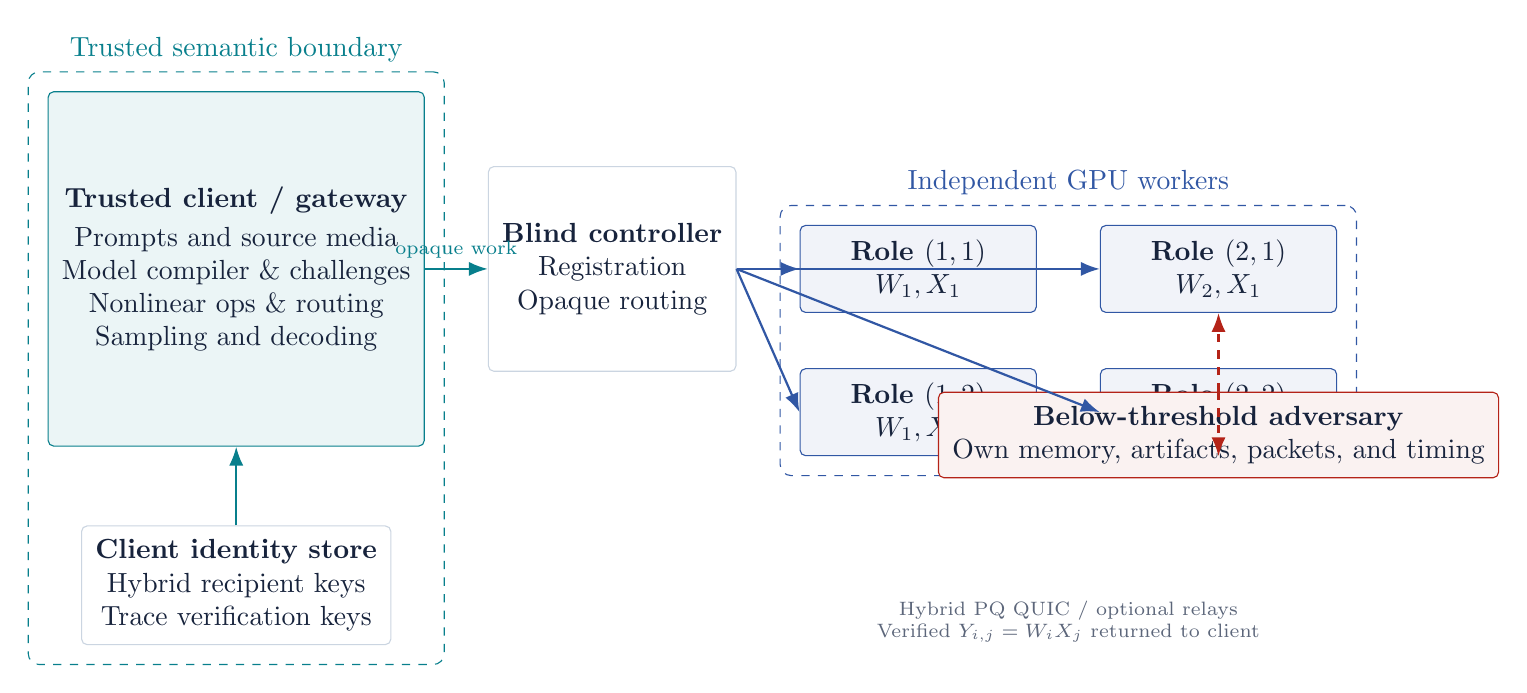
\begin{tikzpicture}[node distance=7mm and 8mm]
\node[trust,minimum width=37mm,minimum height=45mm] (client) {\textbf{Trusted client / gateway}\\[2pt]Prompts and source media\\Model compiler \& challenges\\Nonlinear ops \& routing\\Sampling and decoding};
\node[box,right=of client,minimum width=27mm,minimum height=26mm] (control) {\textbf{Blind controller}\\Registration\\Opaque routing};
\node[worker,right=of control,minimum width=30mm] (w1) {\textbf{Role $(1,1)$}\\$W_1,X_1$};
\node[worker,below=of w1,minimum width=30mm] (w2) {\textbf{Role $(1,2)$}\\$W_1,X_2$};
\node[worker,right=of w1,minimum width=30mm] (w3) {\textbf{Role $(2,1)$}\\$W_2,X_1$};
\node[worker,below=of w3,minimum width=30mm] (w4) {\textbf{Role $(2,2)$}\\$W_2,X_2$};
\node[box,below=10mm of client,minimum width=37mm] (identity) {\textbf{Client identity store}\\Hybrid recipient keys\\Trace verification keys};
\node[danger,below=10mm of w3,minimum width=65mm] (adversary) {\textbf{Below-threshold adversary}\\Own memory, artifacts, packets, and timing};
\begin{scope}[on background layer]
\node[boundary,draw=xteal,fit=(client)(identity),label={[xteal]above:Trusted semantic boundary}] {};
\node[boundary,draw=xblue,fit=(w1)(w2)(w3)(w4),label={[xblue]above:Independent GPU workers}] {};
\end{scope}
\draw[flow,xteal] (client) -- node[above,font=\scriptsize]{opaque work} (control);
\draw[flow,xblue] (control.east) -- (w1.west);
\draw[flow,xblue] (control.east) -- (w2.west);
\draw[flow,xblue] (control.east) -- (w3.west);
\draw[flow,xblue] (control.east) -- (w4.west);
\draw[flow,xteal] (identity) -- (client);
\draw[flow,xred,dashed] (adversary.north) -- (w3.south);
\draw[flow,xred,dashed] (adversary.north) -- (w4.south);
\node[font=\scriptsize,text=xmuted,align=center] at ($(w2.south)!0.5!(w4.south)+(0,-2.1)$) {Hybrid PQ QUIC / optional relays\\Verified $Y_{i,j}=W_iX_j$ returned to client};
\end{tikzpicture}}

\caption{Fortress trust and data boundaries. The client owns model boundaries, nonlinear semantics, and reconstruction. Workers see role-specific shares; relays forward protected frames. Composite TEE evidence is optional on commodity deployments and mandatory in attested mode.}
\label{fig:architecture}
\end{figure}

\subsection{Adversary capabilities}

We consider an active adversary that may fully control one or more below-threshold workers. Such an adversary can read process memory, inspect its assigned artifacts and keys, alter computation, replay packets, delay responses, record timing, and collaborate with other compromised workers. A network adversary can observe and modify traffic, while a malicious relay can inspect its own forwarding metadata. In TEE mode, the cloud operator and host operating system are outside the protected application boundary, but CPU/GPU vendors, firmware, attestation collateral, and verifier implementations remain trust dependencies.

\begin{assumption}[Share non-collusion]\label{assumption:collusion}
For each operation, adversarial workers do not obtain a complementary set of shares sufficient to reconstruct the protected source value. Placement labels and provider diversity are operational aids, not cryptographic proof of independence. Full-grid collusion invalidates the corresponding confidentiality guarantee.
\end{assumption}

\begin{assumption}[Trusted client]\label{assumption:client}
The client or hosted gateway correctly executes tokenization, quantization, nonlinear operations, challenge verification, reconstruction, and output decoding, and protects its long-term and ephemeral secrets. Client compromise is outside the remote-worker confidentiality model.
\end{assumption}

\begin{assumption}[Primitive security]\label{assumption:primitives}
Established cryptographic implementations provide their advertised properties under their respective models. Hybrid key establishment is intended to remain secure unless both component key exchanges fail; it does not make classical TLS certificates post-quantum authentication credentials.
\end{assumption}

\subsection{Security objectives and non-goals}

\Cref{tab:threats} separates confidentiality, integrity, and availability. A system can satisfy one while failing another. In particular, verified incorrect computation does not imply input hiding, and an attested machine can still be malicious at the application layer if its measured workload is not the intended one.

\begin{table}[htbp]
\centering\small
\caption{Threats, controls, and residual exposure.}
\label{tab:threats}
\begin{tabularx}{\linewidth}{>{\raggedright\arraybackslash}p{0.22\linewidth}>{\raggedright\arraybackslash}X>{\raggedright\arraybackslash}p{0.28\linewidth}}
\toprule
\textbf{Adversary action} & \textbf{Primary controls} & \textbf{Residual boundary} \\
\midrule
Read one worker's model state & Additive weight shares; recipient-sealed artifacts; no boundary keys & Complementary-share collusion; reconstruction of seed-expanded shares if the PRG assumption fails \\
Recover user input or output & Client-owned boundaries; activation shares; end-to-end encrypted sessions & Client compromise; complementary-share collusion; semantic side channels \\
Return a wrong matrix product & Independent Freivalds challenges; exact finite-ring arithmetic & Acceptance probability is nonzero; non-matrix and client computation require other controls \\
Replay or alter network traffic & AEAD, sequence tracking, replay windows, directional keys, rotation & Availability attacks and global timing observation \\
Substitute a worker or GPU & Pinned identities, fresh nonce-bound CPU/GPU evidence, workload/image binding & Vendor/verifier compromise and physical attacks \\
Infer workload from traffic & Fixed frames, cover calls, decoy tasks, padded MoE dispatch, relays & Timing, scheduling, cache/TLB, power, and intersection analysis \\
Recover data after release & Stream-ordered scrubbing, KV/latent/state cleanup, host zeroization & Unobservable registers/SRAM, foreign-device memory, root or hypervisor capture before erasure \\
\bottomrule
\end{tabularx}
\end{table}

Availability is intentionally not conflated with confidentiality. Cancellation, bounded request admission, reconnection, and crash recovery improve operational resilience, but a provider can always withhold service. Traffic-analysis resistance is similarly scoped: cover traffic and relays change observable patterns without proving anonymity against a global observer.

\section{Exact arithmetic and additive sharing}\label{sec:arithmetic}

Fortress delegates matrix multiplication rather than an entire transformer layer. This decomposition is the central architectural trade-off: workers receive statistically protected linear operands, while the trusted client retains operations whose nonlinear or routing semantics are difficult to share efficiently.

\subsection{Field and signed representation}

Let $p=2^{32}-5$, which is prime, and let $\field$ be its finite field. Integer encodings produced by a model-specific decoder are canonicalized before sharing. For a field residue $x\in\{0,\ldots,p-1\}$, the signed representative is
\begin{equation}
\operatorname{sgn}(x)=
\begin{cases}
x, & x\leq\lfloor p/2\rfloor,\\
x-p, & \text{otherwise}.
\end{cases}
\label{eq:signed}
\end{equation}
Canonicalization prevents multiple wire representations of the same residue and avoids interpreting a negative two's-complement word as an unrelated field element. Every decoder, transport descriptor, kernel, challenge, and reconstruction path uses the same modulus; mixed-modulus or stale-epoch inputs are rejected.

Products use at least 64-bit intermediates. For $a,b\in[0,p)$, $ab<(2^{32}-5)^2<2^{64}$. The pseudo-Mersenne form permits reduction using $2^{32}\equiv5\pmod p$. Writing $z=z_0+2^{32}z_1$ with $0\leq z_0<2^{32}$ gives
\begin{equation}
z\equiv z_0+5z_1\pmod p,
\end{equation}
followed by repeated folding and a final conditional subtraction. This is exact modular arithmetic, not low-32-bit truncation. Accumulation bounds and supported share counts are checked explicitly; integer wraparound is never presented as exactness.

\subsection{Additive weights and activations}

For $W\in\field^{m\times k}$ and $X\in\field^{k\times n}$, choose $N$ additive shares of each operand:
\begin{equation}
W=\sum_{i=1}^{N}W_i\pmod p,\qquad
X=\sum_{j=1}^{N}X_j\pmod p.
\label{eq:shares}
\end{equation}
For full random sharing, $W_1,\ldots,W_{N-1}$ and $X_1,\ldots,X_{N-1}$ are independent uniform field tensors; the final shares close the sums. By bilinearity,
\begin{align}
Y=WX
&=\left(\sum_iW_i\right)\left(\sum_jX_j\right)\nonumber\\
&=\sum_{i=1}^{N}\sum_{j=1}^{N}Y_{i,j},\qquad Y_{i,j}=W_iX_j\pmod p.
\label{eq:grid}
\end{align}
A role at grid position $(i,j)$ evaluates $Y_{i,j}$ using only $W_i$ and $X_j$. The trusted combiner adds all $N^2$ results in $\field$ and applies signed decoding only after exact reconstruction.

\begin{figure}[htbp]
\centering
\resizebox{0.86\linewidth}{!}{%
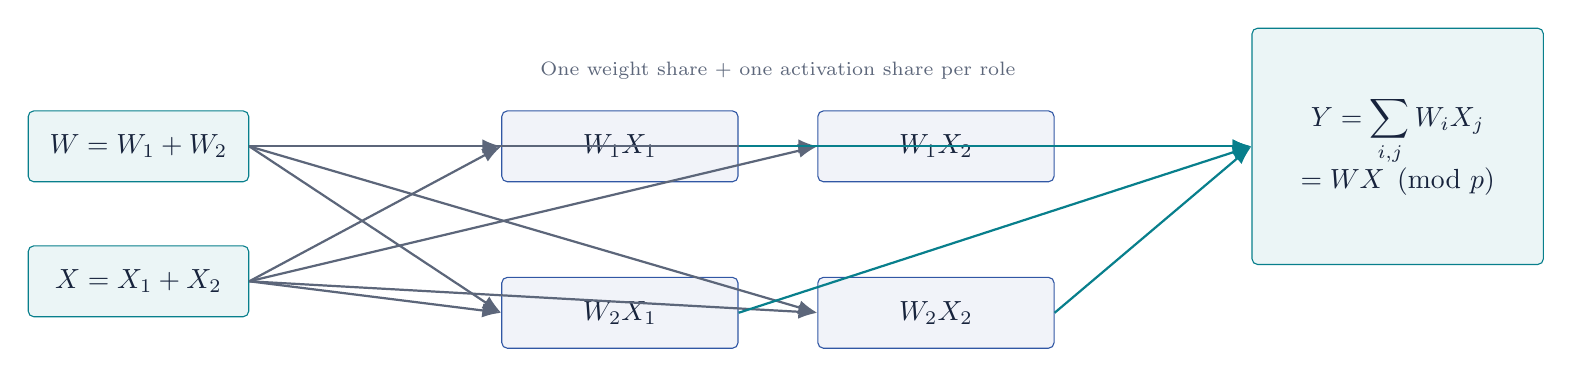
\begin{tikzpicture}[scale=1.0]
\node[trust,minimum width=28mm] (w) {$W=W_1+W_2$};
\node[trust,below=8mm of w,minimum width=28mm] (x) {$X=X_1+X_2$};
\node[worker,right=32mm of w,minimum width=30mm] (a) {$W_1X_1$};
\node[worker,right=10mm of a,minimum width=30mm] (b) {$W_1X_2$};
\node[worker,below=12mm of a,minimum width=30mm] (c) {$W_2X_1$};
\node[worker,below=12mm of b,minimum width=30mm] (d) {$W_2X_2$};
\node[trust,right=25mm of b,minimum width=37mm,minimum height=30mm] (sum) {$Y=\displaystyle\sum_{i,j}W_iX_j$\\$=WX\pmod p$};
\draw[flow] (w.east) -- (a.west); \draw[flow] (w.east) -- (b.west);
\draw[flow] (w.east) -- (c.west); \draw[flow] (w.east) -- (d.west);
\draw[flow] (x.east) -- (a.west); \draw[flow] (x.east) -- (b.west);
\draw[flow] (x.east) -- (c.west); \draw[flow] (x.east) -- (d.west);
\draw[flow,xteal] (a.east) -- (sum.west); \draw[flow,xteal] (b.east) -- (sum.west);
\draw[flow,xteal] (c.east) -- (sum.west); \draw[flow,xteal] (d.east) -- (sum.west);
\node[font=\scriptsize,text=xmuted] at ($(a.north)!0.5!(b.north)+(0,0.5)$) {One weight share + one activation share per role};
\end{tikzpicture}}

\caption{An $N\times N$ operation grid. Each worker receives one weight share and one activation share. Any one share alone is independent of the source under full uniform sharing; reconstruction requires all complementary components.}
\label{fig:share-grid}
\end{figure}

\begin{proposition}[Single-share hiding]\label{prop:hiding}
If all but the closing share are independent and uniform over $\field$, every individual share is uniform and independent of the source. More generally, any subset missing at least one uniformly random, independent component has its distribution unchanged by the source.
\end{proposition}
\begin{proof}[Proof sketch]
For any fixed source $s$ and observed shares, the missing uniform share is a bijection between its possible values and the closing constraint. The conditional distribution of the observed shares therefore remains uniform. Independence across weights and activations extends the argument componentwise.
\end{proof}

This statement is information-theoretic only for full independently generated random shares and under \cref{assumption:collusion}. It says nothing about an adversary that obtains every complementary component, observes the client, or exploits metadata.

\subsection{Seed-expanded storage and transport}

Fortress can derive non-final shares from domain-separated seeds. A 32-byte operation seed is expanded into per-row and per-activation-index seeds; one residual share closes the sum. For model shares, domain separation includes the share index. This reduces material transferred or stored: an experiment with a $16\times16$ matrix recorded 2,048 bytes for two full shares and 1,056 bytes for the seeded representation, saving 992 bytes~\cite{xurcroh-arithmetic}.

\begin{limitation}[Seed expansion is computational]
A seed-expanded share is the output of a pseudorandom generator. It is not an information-theoretic one-time pad, regardless of how many row, role, or operation domains are used. An information-theoretic statement applies only to the full random sharing path with \texttt{seeded\_activations=false}. Task traces record which representation was used.
\end{limitation}

\subsection{Placement and independence}

Correct arithmetic does not itself enforce non-collusion. The compiler emits role-specific artifacts and the placement layer separates complementary components across distinct hosts, countries, CPU vendors, or operators as configured. A model's operations are assigned across several independent role grids, avoiding a single fixed worker population for the whole model. Labels are supplied by the operator and are not independently verified geographic or organizational attestations.

\begin{algorithm}[htbp]
\caption{One shared matrix operation}
\label{alg:grid}
\begin{algorithmic}[1]
\Require Quantized $W,X$; share count $N$; placement policy $\Pi$
\State Canonicalize operands in $\field$ and validate dimensions and overflow bounds
\State Generate or derive $W_1,\ldots,W_N$ and $X_1,\ldots,X_N$ satisfying \cref{eq:shares}
\ForAll{$(i,j)\in[N]\times[N]$}
  \State Select an eligible independent role $(i,j)$ under $\Pi$
  \State Establish or reuse the authenticated role session
  \State Send only role-sealed $W_i$ material and the request-specific $X_j$ share
  \State Receive $Y_{i,j}$ and verify its associated challenges
\EndFor
\State $Y\gets\sum_{i,j}Y_{i,j}\pmod p$
\State Decode signed outputs and pass them to the client-owned nonlinear path
\State \Return $Y$
\end{algorithmic}
\end{algorithm}

Communication grows quadratically in the number of additive shares for a two-operand product. Larger grids increase the number of components that must be pooled but also add network calls, verification work, scheduling overhead, and failure modes. $N$ is therefore a security and deployment parameter, not a free scalability knob.

\section{Verifying delegated linear computation}\label{sec:verification}

Secret sharing hides operands but does not establish that a worker returned the correct product. Fortress therefore attaches challenges derived at compilation time to weight shares. The trusted client knows the unshared challenge relationship; the worker sees only the role material needed for normal execution.

\subsection{Freivalds' algebraic test}

For matrices $A\in\field^{m\times k}$, $B\in\field^{k\times n}$, and a claimed product $C\in\field^{m\times n}$, sample a uniform challenge $r\in\field^n$ and test
\begin{equation}
C r \stackrel{?}{=} A(B r).
\label{eq:freivalds}
\end{equation}
If $C=AB$, equality always holds. If $C\neq AB$, let $D=C-AB\neq0$. Some row $d$ of $D$ is nonzero, and $Dr=0$ requires $d\cdot r=0$.

\begin{theorem}[Freivalds soundness]\label{thm:freivalds}
For one uniformly random $r$, the test in \cref{eq:freivalds} accepts an incorrect $C$ with probability at most $1/p$. With $R$ independently sampled challenges, the acceptance probability is at most $p^{-R}$.
\end{theorem}
\begin{proof}
For a nonzero row $d$, choose a nonzero coordinate $d_h$. Condition on all coordinates except $r_h$. There is at most one value of $r_h$ satisfying $d\cdot r=0$, so the probability is at most $1/p$. Independence gives the $R$-round bound by multiplication.
\end{proof}

The implementation uses fixed challenge material compiled for a model and two independent challenges per weight share on the remote grid path. Fixed challenges avoid regenerating trusted weight products per request, but their lifetime, reuse, and independence must be included in the operational security analysis. A challenge that becomes known to a worker no longer supplies the same assurance. Verification counters are therefore as important as the mathematical primitive: every accepted role result must have been checked.

\begin{figure}[htbp]
\centering
\resizebox{0.91\linewidth}{!}{%
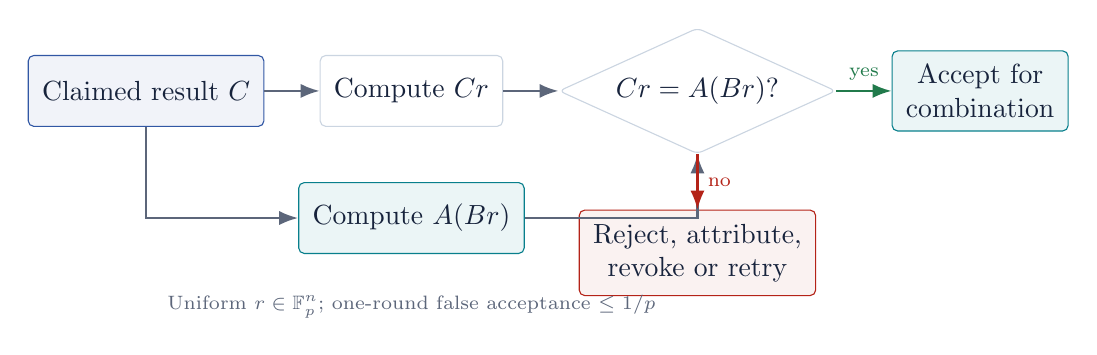
\begin{tikzpicture}[node distance=7mm]
\node[worker] (result) {Claimed result $C$};
\node[box,right=of result] (left) {Compute $Cr$};
\node[trust,below=of left] (right) {Compute $A(Br)$};
\node[box,diamond,aspect=2.2,right=of left,inner sep=3pt] (decision) {$Cr=A(Br)$?};
\node[trust,right=of decision] (accept) {Accept for\\combination};
\node[danger,below=of decision] (reject) {Reject, attribute,\\revoke or retry};
\draw[flow] (result) -- (left);
\draw[flow] (result.south) |- (right.west);
\draw[flow] (left) -- (decision);
\draw[flow] (right.east) -| (decision.south);
\draw[flow,xgreen] (decision) -- node[above,font=\scriptsize]{yes} (accept);
\draw[flow,xred] (decision) -- node[right,font=\scriptsize]{no} (reject);
\node[font=\scriptsize,text=xmuted,below=4mm of right] {Uniform $r\in\mathbb{F}_p^n$; one-round false acceptance $\leq 1/p$};
\end{tikzpicture}}

\caption{Challenge verification and fail-closed recovery. A mismatch invalidates the result; retries preserve operation seeds so retransmission does not change the intended shared computation.}
\label{fig:freivalds}
\end{figure}

\begin{algorithm}[htbp]
\caption{Verified role result}
\label{alg:verify}
\begin{algorithmic}[1]
\Require Claimed $Y_{i,j}$; compiled challenge set $\mathcal{R}$; expected artifact digest
\State Validate frame version, sequence, recipient, tensor shape, and payload length
\State Check the worker checkpoint and pinned artifact digest
\ForAll{$r\in\mathcal{R}$}
  \If{challenge$(Y_{i,j},r)\neq$ expected challenge residue}
    \State Reject the response; attribute the failure; revoke or retry under policy
    \State \Return $\bot$
  \EndIf
\EndFor
\State Increment the verified-result counter and admit $Y_{i,j}$ to the combiner
\State \Return $Y_{i,j}$
\end{algorithmic}
\end{algorithm}

\subsection{Arithmetic-domain boundary}

\begin{securitybox}[Why the bound does not transfer to BF16]
The proof of \cref{thm:freivalds} uses exact equality and uniform challenges over a finite field. BF16, FP16, and FP8 operations round and may reorder accumulation; a small rounding discrepancy is not a field forgery. Fortress therefore asserts the probabilistic bound only for the quantized finite-field path. Reduced-precision implementations require empirical differential tests and explicit numerical tolerances instead.
\end{securitybox}

This distinction also clarifies the evaluation metric. Exact equality to the quantized reference establishes reproducibility of the protected integer computation. It does not imply exact equality to the original BF16 checkpoint. Original-model quality is measured separately using perplexity for text and PSNR or VMAF for generated media.

\subsection{Canaries, checkpoints, and task traces}

A role worker with an identity key signs its loaded artifact digest and a running hash of session traffic. This binds observations to a pinned key and claimed artifact set; it is not hardware attestation. Process canaries associate unique share values with an observer set and trigger attribution and revocation when a monitoring integration reports exposure. A trip identifies the observer set, not necessarily the individual discloser.

Every accepted request can emit a signed task trace containing the model revision, source digest, format, sharing policy, transport group, verification counters, worker checkpoints, and selected resource observations. Traces deliberately exclude prompts and decoded outputs. They make the execution reviewable without turning the evidence system into a plaintext data log.

\section{Protected compilation and execution}\label{sec:runtime}

\subsection{Checkpoint ingestion}

The trusted compiler resolves a model by immutable revision, reads its architecture metadata, verifies the license and checkpoint fingerprint, decodes weights, quantizes supported linear operators, derives role shares, and seals each artifact to a distinct recipient. Architecture detection is checkpoint-driven: model configuration, not a marketing name or an assumed tensor shape, selects the adapter. Unknown graph semantics and unsupported encodings fail closed.

The public compiler accepts Safetensors, GGUF v1--v3, EXL2/GPTQ, and EXL3 containers. GGUF handling covers current tensor type codes, shards, metadata arrays, embedded tokenizers, and both endian modes. EXL2 handles mixed-width groups and activation ordering; EXL3 handles integer and fractional trellis rates, codebooks, and sign/Hadamard restoration. FP8 \texttt{F8\_E4M3} and packed \texttt{I32} decoders were compared against publisher loaders. Container support does not imply universal graph support: an explicit architecture adapter and differential comparison are required.

\begin{figure}[htbp]
\centering
\resizebox{0.96\linewidth}{!}{%
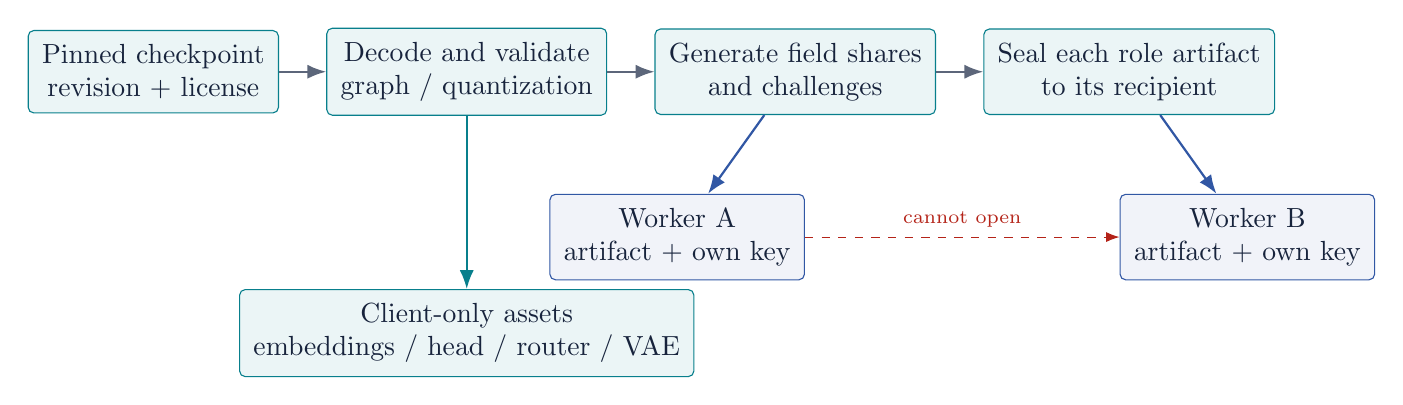
\begin{tikzpicture}[node distance=6mm]
\node[trust] (checkpoint) {Pinned checkpoint\\revision + license};
\node[trust,right=of checkpoint] (decode) {Decode and validate\\graph / quantization};
\node[trust,right=of decode] (share) {Generate field shares\\and challenges};
\node[trust,right=of share] (seal) {Seal each role artifact\\to its recipient};
\node[worker,below=10mm of share,xshift=-15mm] (rolea) {Worker A\\artifact + own key};
\node[worker,below=10mm of seal,xshift=15mm] (roleb) {Worker B\\artifact + own key};
\node[trust,below=10mm of decode,yshift=-12mm,minimum width=40mm] (boundary) {Client-only assets\\embeddings / head / router / VAE};
\draw[flow] (checkpoint) -- (decode); \draw[flow] (decode) -- (share); \draw[flow] (share) -- (seal);
\draw[flow,xblue] (share) -- (rolea); \draw[flow,xblue] (seal) -- (roleb);
\draw[flow,xteal] (decode) -- (boundary);
\draw[-{Latex},xred,dashed] (rolea) -- node[above,font=\scriptsize]{cannot open} (roleb);
\end{tikzpicture}}

\caption{Trusted compilation and recipient isolation. Only role-specific sealed artifacts leave the compiler. Client boundary assets and verification challenges remain under client control.}
\label{fig:compiler}
\end{figure}

\subsection{Quantization and operation extraction}

A neural network can be viewed as an interleaving of linear maps and client-owned semantic operations:
\begin{equation}
h_{\ell+1}=\mathcal{N}_{\ell}\!\left(W_\ell h_\ell;\,\theta_\ell,s_\ell\right),
\end{equation}
where $W_\ell h_\ell$ is delegated, $\mathcal{N}_\ell$ includes normalization, nonlinearities, attention state updates, or routing, and $s_\ell$ denotes client state. The compiler identifies supported matrices in projections, feed-forward blocks, experts, and diffusion backbones. It records tensor shape, source and storage encodings, quantization scale, field modulus, and overflow bounds in authenticated manifests.

For a scalar quantization $W\approx s_W\widetilde{W}$ and $X\approx s_X\widetilde{X}$, the client can reconstruct an approximation using
\begin{equation}
WX\approx s_Ws_X\left(\widetilde{W}\widetilde{X}\right),
\end{equation}
where the inner product is exact in $\field$ and scale restoration is trusted. Model-specific scales and zero points require adapters that preserve the publisher's semantics. The quality impact is empirical and is not inferred from the zero integer-reference error.

\subsection{Role artifacts and key separation}

A manifest identifies the model, graph, field, operation, recipient, and artifact digests. Each role's data key is sealed to a distinct hybrid recipient identity. Client embeddings, language-model head, router state, challenge vectors, bases, VAEs, and decoders are separately protected and never included in ordinary worker artifacts. Workers cannot use their own recipient identity to open another role's envelope.

This credential separation does not assert that an arbitrary algebraic weight transformation is irreversible. Earlier obfuscation-first mechanisms remain useful as inner layers and transition tools, but Fortress production execution relies on additive sharing rather than treating an orthogonal matrix as encryption.

\subsection{Trusted combiner and model state}

The combiner reconstructs each linear result, checks verification counters, and executes operations withheld from workers. For text, these include tokenization, embeddings, normalization, attention mixing and state ownership, expert routing, sampling, and final decoding. For MoE models, padded dropless dispatch gives every expert a constant workload and assigns dummy results zero combination weight. This reduces selection-dependent network volume without eliminating timing or microarchitectural leakage.

A single \texttt{FortressGridRuntime} per model shares one authenticated connection and encrypted session per role across operations. This avoids creating one thread pool, cover loop, and connection per matrix. Operation names remain inside authenticated payloads; fresh seeds and retry-stable derivation prevent retransmission from silently changing the computation. Session rotation and cancellation are role-scoped.

\subsection{Memory lifecycle}

Fortress treats logical deallocation and physical sanitization as different operations. Sensitive host staging uses wipeable buffers; role activation, transport, latent, and recurrent buffers are cleaned at request or session boundaries. On CUDA, zero-on-free schedules the wipe on the allocation's stream and synchronizes before reuse. KV pools require physical-slot wipes because returning a logical block need not invoke the allocator.

\begin{figure}[htbp]
\centering
\resizebox{0.96\linewidth}{!}{%
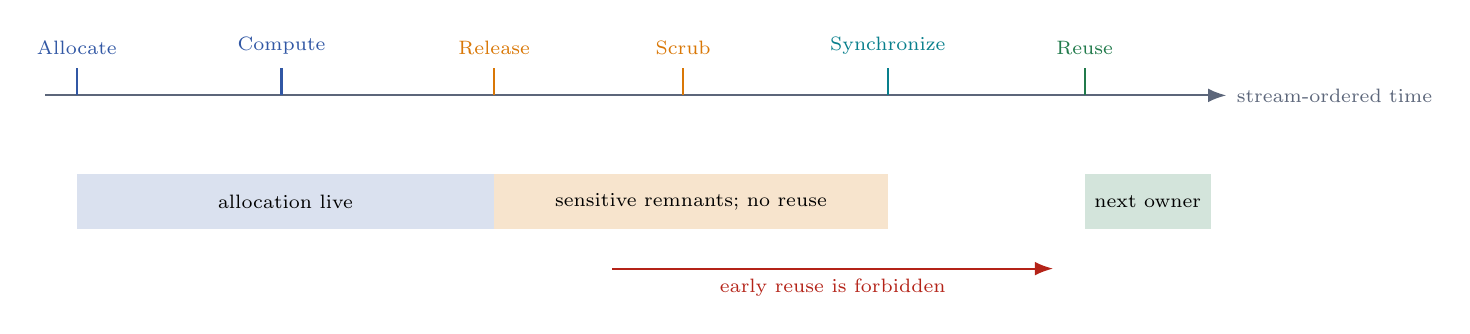
\begin{tikzpicture}[x=1.0cm,y=1.0cm]
\draw[-{Latex},thick,xmuted] (0,0) -- (15,0) node[right,font=\scriptsize]{stream-ordered time};
\foreach \x/\name/\colour in {0.4/Allocate/xblue,3.0/Compute/xblue,5.7/Release/xorange,8.1/Scrub/xorange,10.7/Synchronize/xteal,13.2/Reuse/xgreen} {
  \draw[thick,\colour] (\x,0) -- (\x,0.35);
  \node[above,font=\scriptsize,text=\colour,align=center] at (\x,0.4) {\name};
}
\fill[xblue!18] (0.4,-1.0) rectangle (5.7,-1.7);
\fill[xorange!20] (5.7,-1.0) rectangle (10.7,-1.7);
\fill[xgreen!20] (13.2,-1.0) rectangle (14.8,-1.7);
\node[font=\scriptsize] at (3.05,-1.35) {allocation live};
\node[font=\scriptsize] at (8.2,-1.35) {sensitive remnants; no reuse};
\node[font=\scriptsize] at (14,-1.35) {next owner};
\draw[xred,thick,-{Latex}] (7.2,-2.2) -- node[below,font=\scriptsize]{early reuse is forbidden} (12.8,-2.2);
\end{tikzpicture}}

\caption{Wipe-before-reuse ordering. Stream synchronization makes the tested allocation unavailable to the next owner until scrubbing completes; this does not prove erasure of every register or SRAM location.}
\label{fig:memory}
\end{figure}

\begin{limitation}[Scope of memory evidence]
An independent epilogue kernel cannot establish that every physical register, all shared memory, or another device's memory has been cleared. Python and framework copies, host root access, hypervisors, and capture before erasure remain relevant. The hardware evidence concerns measured allocation and cleanup behavior, not universal physical erasure.
\end{limitation}

\subsection{Failure behavior}

Strict mode has no silent plaintext fallback. Missing adapters, incompatible revisions, invalid evidence, malformed tensor descriptors, stale epochs, and unsupported model semantics stop execution. Cancellation and monotonic deadlines are checked between denoising steps and between additive-grid rows. This cooperative mechanism does not claim preemption inside an arbitrary third-party native kernel. Shutdown cancels active work, waits for in-flight cleanup, and retains recovery state if remote teardown fails.

\section{Secure transport and evidence}\label{sec:transport}

\subsection{Layered protection}

Fortress transport has three distinct layers. Rust QUIC supplies authenticated, encrypted, forward-secret links using TLS 1.3~\cite{rfc9000,rfc8446}. The role-session protocol establishes an end-to-end application session using hybrid HPKE. Fixed-size binary frames then carry tensor descriptors and encrypted role payloads with explicit version, sequence, type, shape, and length fields.

The hybrid suite combines X25519 and ML-KEM-768, HKDF-SHA256, and ChaCha20-Poly1305~\cite{rfc9180,fips203,rfc8439}. ML-KEM is the NIST-standardized module-lattice key-encapsulation mechanism derived from CRYSTALS-Kyber~\cite{kyber}. The purpose of the combination is to retain confidentiality unless both key-exchange components fail, subject to a correct combiner and implementation.

\subsection{Role-session establishment}

Let $K_w$ be a worker's static hybrid recipient public key. The client creates an ephemeral key pair and sends a fresh ephemeral public value with a secret $s_c$ sealed to $K_w$. The worker opens $s_c$, seals its own secret $s_w$ to the client's ephemeral key, and returns it with its loaded-artifact digest and, when configured, a signature over the exchange transcript $T$. Both parties derive
\begin{equation}
k_0=\HKDF(s_c\,\|\,s_w,\ \text{salt}=H(T),\ \text{info}=\texttt{Fortress role session}),
\end{equation}
followed by directional send/receive keys. On direct routes, a TLS exporter is mixed into the handshake so a transcript cannot be moved to another TLS connection. A relayed route has no shared client--worker TLS session and therefore reports that binding as absent.

Rotation replaces a session key using a one-way derivation and starts a new nonce domain:
\begin{equation}
k_{e+1}=\HKDF(k_e,\ \text{info}=\texttt{rotation}\,\|\,e+1).
\end{equation}
The worker's static key alone should not open a recorded session because the worker secret was sealed to a discarded client ephemeral key. Python cannot guarantee immediate erasure of every discarded byte; forward secrecy is consequently a protocol property with best-effort implementation hygiene, not proof of physical memory erasure.

\begin{figure}[htbp]
\centering
\resizebox{0.85\linewidth}{!}{%
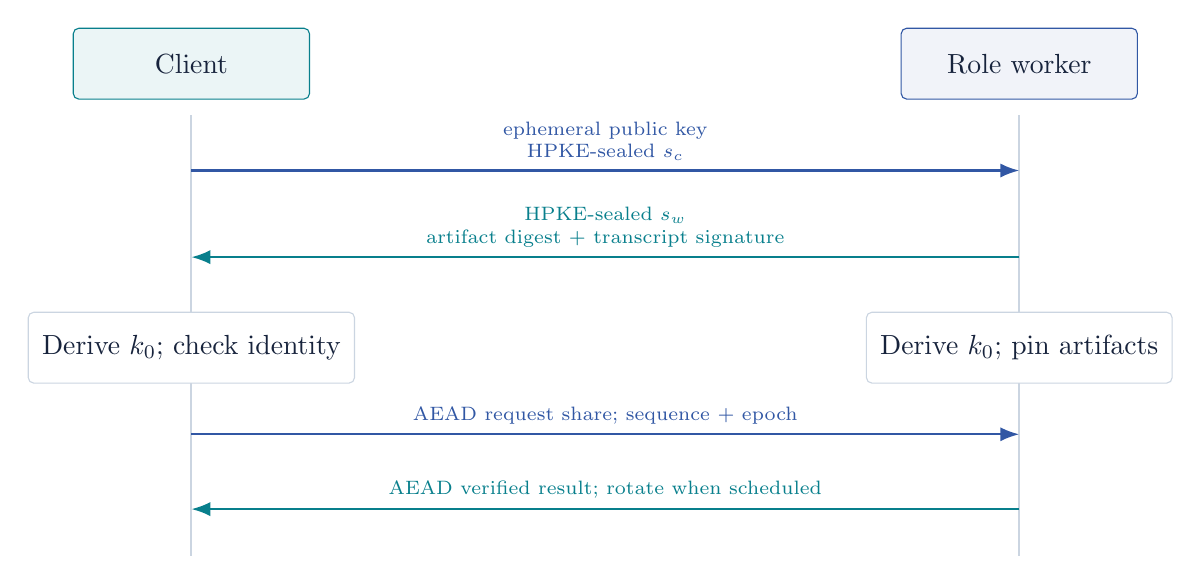
\begin{tikzpicture}
\node[trust,minimum width=30mm] (client) {Client};
\node[worker,right=75mm of client,minimum width=30mm] (worker) {Role worker};
\draw[thick,xline] ($(client.south)+(0,-0.2)$) -- ++(0,-5.6);
\draw[thick,xline] ($(worker.south)+(0,-0.2)$) -- ++(0,-5.6);
\draw[flow,xblue] ($(client.south)+(0,-0.9)$) -- node[above,font=\scriptsize,align=center]{ephemeral public key\\HPKE-sealed $s_c$} ($(worker.south)+(0,-0.9)$);
\draw[flow,xteal] ($(worker.south)+(0,-2.0)$) -- node[above,font=\scriptsize,align=center]{HPKE-sealed $s_w$\\artifact digest + transcript signature} ($(client.south)+(0,-2.0)$);
\node[box] at ($(client.south)+(0,-3.15)$) {Derive $k_0$; check identity};
\node[box] at ($(worker.south)+(0,-3.15)$) {Derive $k_0$; pin artifacts};
\draw[flow,xblue] ($(client.south)+(0,-4.25)$) -- node[above,font=\scriptsize]{AEAD request share; sequence + epoch} ($(worker.south)+(0,-4.25)$);
\draw[flow,xteal] ($(worker.south)+(0,-5.2)$) -- node[above,font=\scriptsize]{AEAD verified result; rotate when scheduled} ($(client.south)+(0,-5.2)$);
\end{tikzpicture}}

\caption{Fortress role-session establishment. The application session remains end-to-end across relays. Worker identity, artifact digest, challenge freshness, and directional keys have separate purposes.}
\label{fig:session}
\end{figure}

\subsection{Framing, replay, and return paths}

AEAD nonces are monotonic within a key epoch. Directional HKDF contexts prevent accidental reuse of the same application key in both directions. The receiver maintains a 64-sequence replay window: recent reordering is accepted, duplicates and excessively old packets are rejected, and nonce exhaustion fails closed. Bounded binary parsing rejects unsupported versions, malformed lengths, trailing bytes, and integer overflow without panics.

Onion routing wraps each request layer to one authorized hop. A relay learns its next address but not the application session keys. The response is protected by the end-to-end role session and forwarded unchanged. One relay observes both endpoints; meaningful client--worker endpoint separation requires at least two non-colluding relays. Tor and I2P carriers instead frame QUIC datagrams over their respective stream transports, preserving mutual TLS and the application session inside the carrier. Neither design defeats global timing and volume correlation.

Cover calls use the same frame form and length as real calls. Constant-rate mode fills unused slots, while decoy tasks execute complete requests whose outputs are discarded. These mechanisms impose throughput and latency costs. They do not hide the identities of contacted workers, and operation order can still reveal model structure.

\subsection{Hardware evidence}

Attested mode requires fresh evidence bound to a challenge nonce, workload and artifact identities, recipient key, and expected image measurement. AMD SEV-SNP and Intel TDX evidence covers the CPU/virtual-machine side; NVIDIA evidence covers the GPU side. Composite acceptance requires both. The client rejects stale quotes, wrong evidence, second-GPU substitution, and changed image measurements rather than downgrading to commodity execution.

Provider APIs and virtual-machine names are not evidence. A successful create/destroy lifecycle proves only that the provider control plane behaved as observed. Physical attestation requires vendor-signed fields, current collateral, and policy evaluation. The vendor, firmware, and verifier remain additional trust roots.

\subsection{Signed evidence and transparency}

Task traces, model manifests, release manifests, worker registrations, and ladder evidence use Ed25519 and ML-DSA-65 together; both signatures must verify~\cite{fips204}. ML-DSA is the NIST-standardized module-lattice signature derived from CRYSTALS-Dilithium~\cite{dilithium}. Validation evidence blocks form a hash chain from F0 and M0 through the text/media rungs and attested executions. Each accepted rung binds the preceding result, source identity, model revision, and verification counters.

\begin{figure}[htbp]
\centering
\resizebox{0.94\linewidth}{!}{%
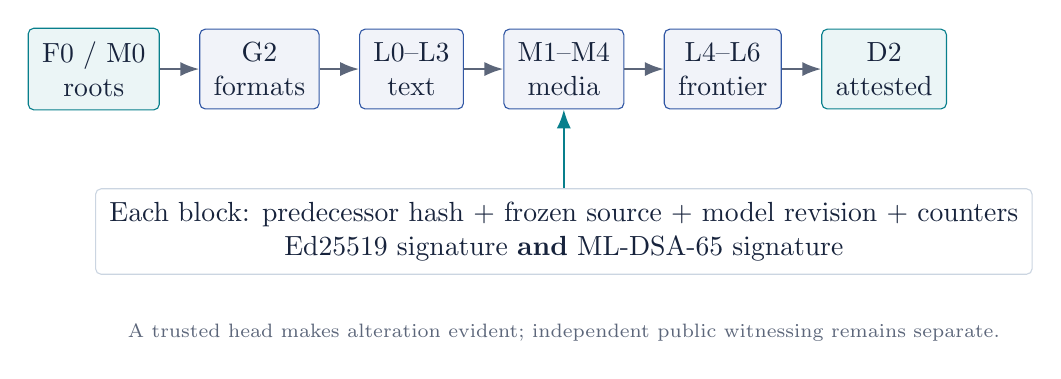
\begin{tikzpicture}[node distance=5mm]
\node[trust] (f0) {F0 / M0\\roots};
\node[worker,right=of f0] (g2) {G2\\formats};
\node[worker,right=of g2] (l0) {L0--L3\\text};
\node[worker,right=of l0] (m1) {M1--M4\\media};
\node[worker,right=of m1] (l4) {L4--L6\\frontier};
\node[trust,right=of l4] (d2) {D2\\attested};
\draw[flow] (f0) -- (g2); \draw[flow] (g2) -- (l0); \draw[flow] (l0) -- (m1); \draw[flow] (m1) -- (l4); \draw[flow] (l4) -- (d2);
\node[box,below=10mm of m1,minimum width=80mm] (sign) {Each block: predecessor hash + frozen source + model revision + counters\\Ed25519 signature \textbf{and} ML-DSA-65 signature};
\draw[flow,xteal] (sign) -- (m1);
\node[font=\scriptsize,text=xmuted,below=5mm of sign] {A trusted head makes alteration evident; independent public witnessing remains separate.};
\end{tikzpicture}}

\caption{Tamper-evident validation and request evidence. Dual signatures authenticate records; hash chaining detects modification or removal relative to a trusted head. Independent witnessing remains an external assurance activity.}
\label{fig:evidence}
\end{figure}

An append-only Merkle digest log supports inclusion and consistency proofs for traces, model manifests, and releases. The project does not itself operate an independent public witness. A log and a witness run by the same party do not provide independent equivocation detection, and a signed trace is evidence about an asserted execution rather than a cryptographic proof of an entire neural-network forward pass.

\section{Unified multimodal inference}\label{sec:multimodal}

Fortress applies the same sharing, transport, verification, and evidence infrastructure to text, vision-language conditioning, image diffusion, and video generation. Modal adapters differ in graph extraction and client boundary, not in whether workers are trusted with plaintext.

\subsection{Dense and mixture-of-experts language models}

For a transformer decoder, tokenization and embedding remain client-owned. Supported linear projections are quantized and delegated; the combiner applies normalization, attention semantics, residual updates, and nonlinearities. The final normalization, language-model head, and sampling stay at the client. This supports synchronous, asynchronous, and streaming generation under one request state machine.

An MoE block computes
\begin{equation}
y=\sum_{e\in\operatorname{TopK}(r(x))}g_e(x)E_e(x),
\end{equation}
where the router $r$ and gates $g$ remain trusted. Protected dispatch sends a fixed-capacity workload to every selected execution domain, adds dummy items when needed, and sets dummy output weights to zero:
\begin{equation}
y=\sum_e g_e(x)E_e(x)\,\mathbf{1}[e\text{ is real}].
\end{equation}
Decoy expert calls and constant-load padding reduce direct packet-volume leakage, but do not remove timing, access-pattern, cache, TLB, or power channels. Large MoE models additionally benefit from measured expert placement and client-side routers that never become worker-visible model state.

The L5 evaluation exercised GLM-5.3-Flash with 288 experts across 45 layers. The L6 evaluation used Kimi-K2.6 with measured REAP expert pruning: all 61 layers and 384 experts per layer were measured before pruning, the retained fraction was 0.472, and quality was compared with the unpruned original on a separate trusted reference host~\cite{xurcroh-validation}.

\subsection{Vision-language conditioning}

VLM inputs are prepared at the trusted boundary. Image patches, supported audio embeddings, text tokens, masks, and positional information are assembled before protected execution. Chaff tokens are explicitly attention-masked so they cannot alter model semantics. Model-specific configuration is derived from the pinned checkpoint; unsupported positional, recurrence, or graph variants are rejected rather than approximated by a generic adapter.

The Qwen 3.8 27B rung included image/audio conditioning substeps with exact quantized-reference equality. This is evidence for the evaluated adapter and revision, not a claim that every future VLM can be handled by the same tensor layout.

\subsection{Image generation and editing}

A diffusion transformer produces a sequence of protected latent updates. The trusted client generates or imports initial noise, encodes source images for image-to-image workflows, controls the scheduler, and decodes final latents with a VAE or lightweight decoder. A flow-matching update can be written
\begin{equation}
z_{t+1}=z_t+\Delta_t\,v_\theta(z_t,c,t),
\end{equation}
where $c$ is conditioning and $v_\theta$ contains delegated linear operations interleaved with trusted nonlinear and scheduling operations. Masked editing constrains the reconstruction region at the client rather than exposing the original image to workers.

For an equivariant transition layer used by the compiler, a linear map satisfies
\begin{equation}
\widehat{W}=U_{\mathrm{out}}WU_{\mathrm{in}}^{-1},\qquad
\widehat{W}\widehat{x}=U_{\mathrm{out}}Wx
\quad\text{when}\quad \widehat{x}=U_{\mathrm{in}}x.
\label{eq:equivariance}
\end{equation}
Such a transformation demonstrates functional equivalence, not confidentiality. Orthogonal transformations preserve inner products and norms and may permit alignment against public models. Fortress consequently treats them as an inner compilation layer only.

Adaptive layer normalization introduces coefficient-specific constraints. If $P$ is a signed permutation, multiplicative $\gamma$ and $\alpha$ coefficients require unsigned permutations while additive $\beta$ coefficients use the signed form; applying signs uniformly breaks products whose signs cancel. The compiler validates joint attention, modulation, feed-forward paths, and input/output projections before emitting media artifacts. Worker requests do not carry the client basis or spatial permutation.

\subsection{Video and audio}

Video adds temporal token structure, recurrent state, frame scheduling, and optional audio. The client retains the initial media, temporal mask semantics, final latent reconstruction, VAE decoding, and MP4/audio encoding. Protected workers evaluate supported matrix operations without receiving decoded frames. Recurrent state is transformed and cleaned according to the same request-scoped ownership rules as text KV state and image latents.

The media ladder exercised Wan 2.2 text/image-to-video, LTX-2.5, and MiniMax H3 recurrent-state and joint-audio paths. Exact latent equality and deterministic output checks are reported alongside VMAF; neither metric alone measures every aspect of perceptual quality.

\begin{figure}[htbp]
\centering
\resizebox{0.96\linewidth}{!}{%
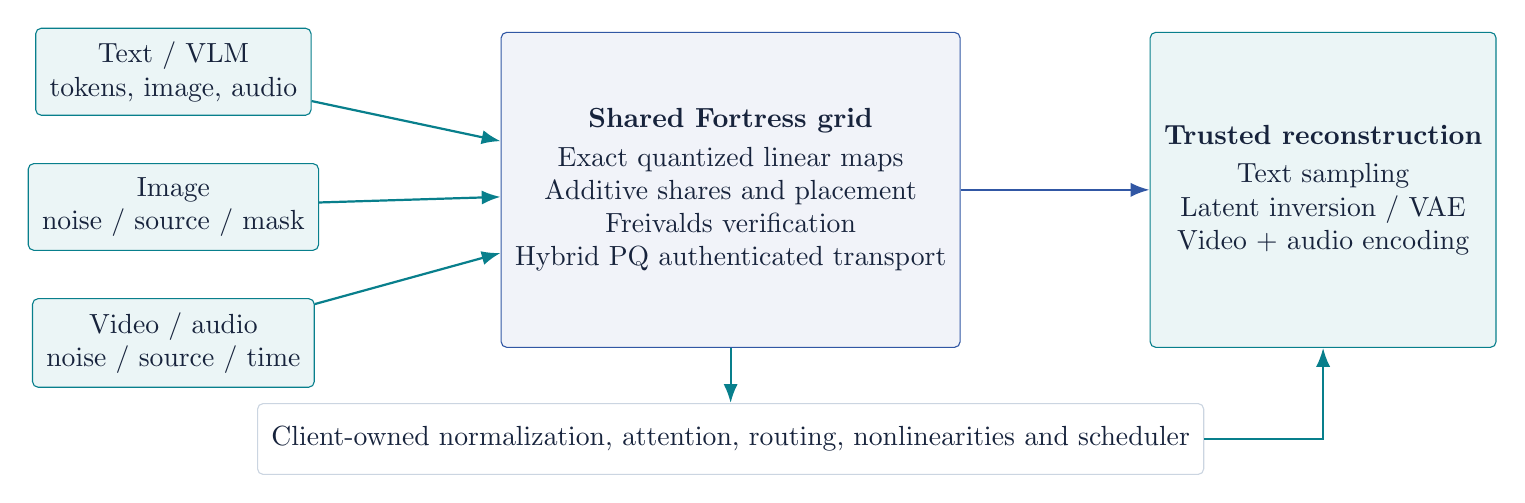
\begin{tikzpicture}[node distance=6mm and 7mm]
\node[trust,minimum width=29mm] (text) {Text / VLM\\tokens, image, audio};
\node[trust,below=of text,minimum width=29mm] (image) {Image\\noise / source / mask};
\node[trust,below=of image,minimum width=29mm] (video) {Video / audio\\noise / source / time};
\node[worker,right=24mm of text,yshift=-15mm,minimum width=50mm,minimum height=40mm] (grid) {\textbf{Shared Fortress grid}\\[2pt]Exact quantized linear maps\\Additive shares and placement\\Freivalds verification\\Hybrid PQ authenticated transport};
\node[trust,right=24mm of grid,minimum width=33mm,minimum height=40mm] (output) {\textbf{Trusted reconstruction}\\[2pt]Text sampling\\Latent inversion / VAE\\Video + audio encoding};
\draw[flow,xteal] (text) -- (grid); \draw[flow,xteal] (image) -- (grid); \draw[flow,xteal] (video) -- (grid);
\draw[flow,xblue] (grid) -- (output);
\node[box,below=7mm of grid,minimum width=65mm] (client) {Client-owned normalization, attention, routing, nonlinearities and scheduler};
\draw[flow,xteal] (grid) -- (client); \draw[flow,xteal] (client) -| (output);
\end{tikzpicture}}

\caption{Unified Fortress dataflow. Modality-specific encoders and decoders stay at the trusted boundary, while the shared grid executes verified linear operations.}
\label{fig:multimodal}
\end{figure}

\section{Implementation and reproducibility}\label{sec:implementation}

\subsection{Polyglot component boundaries}

Xurcroh assigns implementation languages according to their operational role. Python implements the public SDK, model ingestion, trusted combiner, orchestration integration, and provider lifecycle. Rust owns bounded protocol parsing, AEAD, session state, and QUIC transport. C++ and CUDA implement native memory operations and exact field kernels. TypeScript implements an independent interactive manual whose simulations are not used in production inference.

These components share versioned schemas and explicit ownership rules. The Rust protocol is used by native Python bindings rather than maintaining a second wire serializer. GPU tensors cross language boundaries with explicit shape, dtype, lifetime, synchronization, and cleanup contracts. Optional integrations import framework code only at runtime and reject incompatible pinned APIs.

The Fortress production path supersedes the earlier obfuscation-first vLLM/SGLang design for protected inference. Existing vLLM, SGLang, and xDiT integrations remain numerical references and transition tools; launching an ordinary plaintext model server is not accepted as Fortress execution.

\subsection{Deployment topology}

SDK-managed deployment discovers host capacity, resolves a pinned checkpoint, compiles role artifacts on trusted infrastructure, deploys the committed source, bootstraps a minimal CUDA environment, generates deployment-scoped mutual-TLS identities, and starts role workers. Startup concurrency is bounded to avoid overwhelming a small gateway. A datagram relay supports providers where direct UDP is unavailable, with end-to-end QUIC and application cryptography retained inside the SSH tunnel.

For an $N$-share two-operand operation, placement uses $N^2$ roles. A default Gemma configuration uses five operation groups and thus $5N^2$ independently addressable hosts; $N=2$ yields 20 hosts. This is a topology rule, not an assertion that arbitrary models fit. \texttt{client.preflight()} checks the actual checkpoint, role memory, host count, file descriptors, and bandwidth requirements before execution.

Provider adapters expose offer discovery, creation, destruction, remaining-resource checks, and charge reporting. Vast.ai supplies bounded validation lifecycle automation; RunPod and other SSH hosts use the managed-worker path. Azure, Google Cloud, and Alibaba Cloud have confidential-GPU adapters. OCI, AWS Nitro, and IBM paths are CPU-only and cannot be presented as confidential GPU execution.

\subsection{Verification tooling}

The repository includes Python unit and integration tests, Rust tests and linting, native CUDA tests, protocol fuzzing, symbolic ProVerif models, numerical differential tests, container checks, dependency/secret scanning, and frontend tests for the manual. Benchmark commands emit versioned JSON and omit prompts, outputs, media, credentials, and keys.

Local benchmark commands execute real algorithms or public SDK requests. They do not generate synthetic inference responses. The interactive manual, by contrast, is explicitly a browser-based educational simulation; it is not cited as hardware evidence.

\subsection{Artifact scope}

The primary artifact is available at \url{https://github.com/Shannon-Tool/Xurcroh}. The public model matrix pins official checkpoint revisions and licenses~\cite{xurcroh-models}. The hardware report records frozen source identity and evidence hashes~\cite{xurcroh-validation}. This paper's CSV files and plotting script make its figures regenerable from the published aggregate values.

\begin{evidencebox}[Reproducibility statement]
The manuscript sources, plots, and public documentation are reproducible from the repository. Independent reproduction of the frozen hardware ladder, second-party release builds, and an independently operated transparency witness remain external work. A matching wheel hash from two builds by the same party is useful engineering evidence but is not second-party reproducibility.
\end{evidencebox}

\section{Evaluation}\label{sec:evaluation}

The public validation program evaluated protected execution on physical GPUs across independent hosts. Every accepted rung required exact equality to the Fortress quantized reference, separate source-model quality measurement, 34 worker-compromise and transport checks, zero Freivalds failures, canary attribution and revocation, verified task traces, streaming/cancellation/concurrency/recovery, resource measurement, signed chained evidence, cost accounting, and teardown proof. Results below are from \frozenbuild{} (\texttt{7f31c2e0}) and are historical measurements, not performance guarantees~\cite{xurcroh-validation}.

\subsection{Text and VLM ladder}

\begin{table}[htbp]
\centering\scriptsize
\caption{Physical text ladder. Quality is perplexity delta over 10,000 public prompts against the original model; L6 compares against the unpruned original. All rows have zero maximum absolute error against the Fortress quantized reference.}
\label{tab:text-ladder}
\resizebox{\linewidth}{!}{%
\begin{tabularx}{\linewidth}{l>{\raggedright\arraybackslash}X>{\raggedright\arraybackslash}p{0.26\linewidth}rrrr}
\toprule
\textbf{Rung} & \textbf{Model} & \textbf{Fleet} & \textbf{Hosts} & \textbf{Quality} & \textbf{VRAM/role} & \textbf{Cost} \\
 & & & & \textbf{(\%)} & \textbf{(GB)} & \textbf{(USD)} \\
\midrule
L0 & Gemma 4 E2B & 4$\times$ RTX 4090 & 4 & 2.1 & 17.1 & 57.94 \\
L1a & Gemma 4 E4B & 4$\times$ RTX 4090 & 4 & 1.8 & 26.8 & 84.31 \\
L1b & Gemma 4 12B & 4$\times$ A100 PCIe & 4 & 1.7 & 42.3 & 92.51 \\
L2 & Gemma 4 26B-A4B & 8$\times$ A100 PCIe & 8 & 2.4 & 61.0 & 302.51 \\
L3a & Gemma 4 31B & 8$\times$ A100 PCIe & 8 & 1.9 & 68.9 & 291.06 \\
L3b & Qwen 3.8 27B & 8$\times$ A100 PCIe & 8 & 2.0 & 64.2 & 286.90 \\
L4 & Mistral Medium 3.5 128B & 24$\times$ H100 PCIe + 8$\times$ H100 SXM & 32 & 2.6 & 63.2 & 2,735.16 \\
L5 & GLM-5.3-Flash & 62$\times$ H100 PCIe + 14$\times$ H100 SXM & 76 & 2.9 & 58.9 & 6,522.80 \\
L6 & Kimi-K2.6, REAP 0.472 & 84$\times$ H100 PCIe + 36$\times$ H100 SXM & 120 & 4.1 & 56.4 & 10,467.97 \\
\bottomrule
\end{tabularx}}
\end{table}

\Cref{tab:text-ladder} spans compact dense models, VLM conditioning, FP8 and packed-integer formats, and large MoE fleets. L2 was the first evaluated MoE rung with client routers, decoy expert calls, and padded dispatch. L5 and L6 passed eight-host rehearsals before full-fleet execution. Seed expansion operated on every rented GPU, and the listed VRAM values are measured per-role peaks rather than analytical four-byte upper bounds.

\begin{figure}[htbp]
\centering
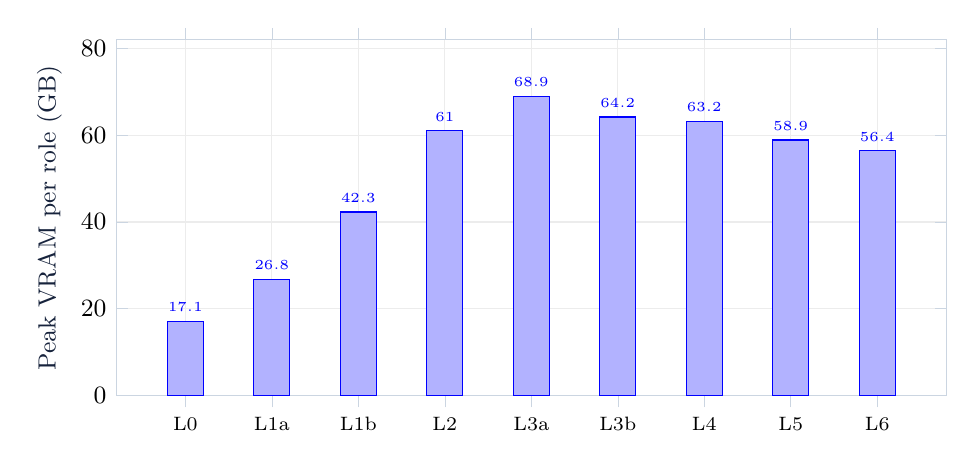
\begin{tikzpicture}
\begin{axis}[width=\columnwidth,height=6.1cm,ybar,bar width=13pt,symbolic x coords={L0,L1a,L1b,L2,L3a,L3b,L4,L5,L6},xtick=data,x tick label style={font=\scriptsize},ylabel={Peak VRAM per role (GB)},ymin=0,ymax=82,grid=major,grid style={gray!15},nodes near coords,nodes near coords style={font=\tiny},every axis plot/.append style={fill=xblue!80,draw=xblue}]
\addplot coordinates {
(L0,17.1)
(L1a,26.8)
(L1b,42.3)
(L2,61.0)
(L3a,68.9)
(L3b,64.2)
(L4,63.2)
(L5,58.9)
(L6,56.4)
};
\end{axis}
\end{tikzpicture}
\caption{Measured peak VRAM per role across the physical text ladder. Larger fleets do not imply monotonically increasing per-role memory because model graph, quantization, and role assignment differ.}
\label{fig:text-resources}
\end{figure}

\begin{figure}[htbp]
\centering
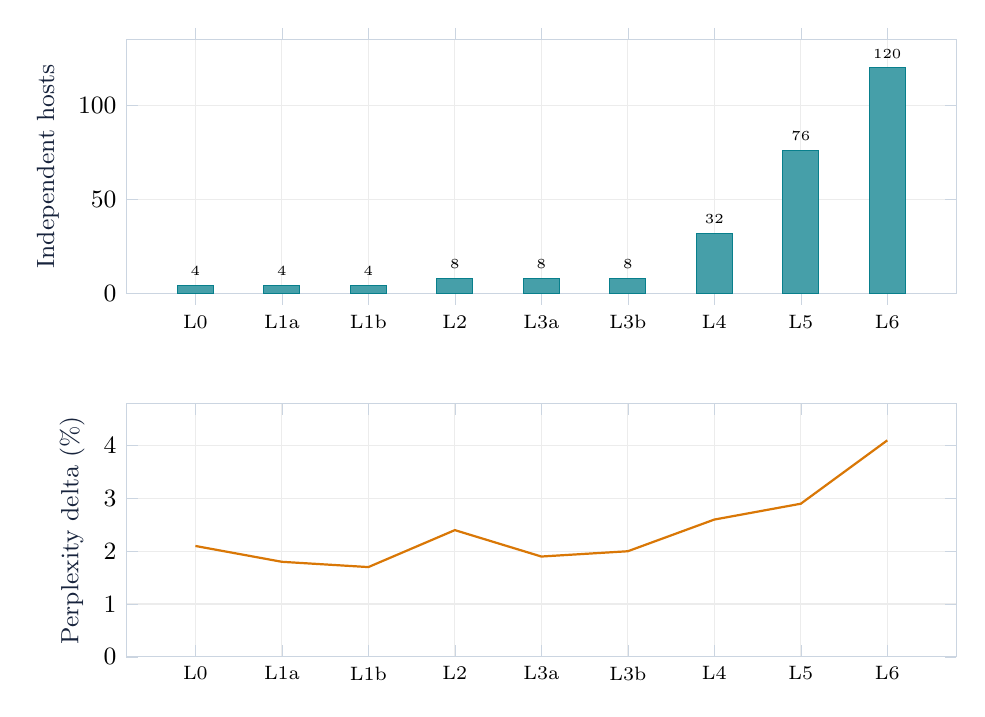
\begin{tikzpicture}
\begin{groupplot}[group style={group size=1 by 2,vertical sep=1.4cm},width=\columnwidth,height=4.8cm,symbolic x coords={L0,L1a,L1b,L2,L3a,L3b,L4,L5,L6},xtick=data,x tick label style={font=\scriptsize},grid=major,grid style={gray!15}]
\nextgroupplot[ybar,bar width=13pt,ylabel={Independent hosts},ymin=0,ymax=135,nodes near coords,nodes near coords style={font=\tiny}]
\addplot[fill=xteal!75,draw=xteal] coordinates {
(L0,4)
(L1a,4)
(L1b,4)
(L2,8)
(L3a,8)
(L3b,8)
(L4,32)
(L5,76)
(L6,120)
};
\nextgroupplot[ylabel={Perplexity delta (\%)},ymin=0,ymax=4.8,ytick={0,1,2,3,4},mark=*,mark size=1.8pt]
\addplot[xorange,thick] coordinates {
(L0,2.1)
(L1a,1.8)
(L1b,1.7)
(L2,2.4)
(L3a,1.9)
(L3b,2.0)
(L4,2.6)
(L5,2.9)
(L6,4.1)
};
\end{groupplot}
\end{tikzpicture}
\caption{Independent fleet size and measured perplexity delta. Quality is not a pass/fail threshold. L6's 4.1\% delta is relative to the unpruned model and includes the effect of REAP pruning.}
\label{fig:fleet-quality}
\end{figure}

The L6 record reports 184,224 role requests and 184,224 verified results, a client RSS peak of 71.2 GB, peak role VRAM of 56.4 GB, 88.2 GiB/min bandwidth, and median operation latency of 1,411 ms. These observations describe one large protected configuration and its client-heavy arithmetic decomposition; they must not be repackaged as generic tokens-per-second estimates.

\subsection{Image and video ladder}

\begin{table}[htbp]
\centering\small
\caption{Physical media ladder. Every workflow has exact local-versus-grid latent equality. Costs are totals for the indicated M1--M4 rung, not individual model prices.}
\label{tab:media-ladder}
\begin{tabularx}{\linewidth}{ll>{\raggedright\arraybackslash}Xrr}
\toprule
\textbf{Rung} & \textbf{Model} & \textbf{Validated workflows} & \textbf{Quality} & \textbf{Rung cost (USD)} \\
\midrule
M1a & FLUX.2 klein 4B & Text-to-image; non-square/odd shapes & 44.2 dB PSNR & \multirow{2}{*}{124.62} \\
M1b & Z-Image-Turbo & Few-step text-to-image & 43.7 dB PSNR & \\
\midrule
M2a & Qwen-Image 2.1 & T2I, I2I, masked editing & 42.8 dB PSNR & \multirow{2}{*}{412.85} \\
M2b & FLUX.2-dev & T2I, I2I, masked editing & 42.1 dB PSNR & \\
\midrule
M3a & Wan 2.2 TI2V 5B & Text/image-to-video; deterministic MP4 & 96.4 VMAF & \multirow{2}{*}{401.79} \\
M3b & LTX-2.5 & Video generation & 95.8 VMAF & \\
\midrule
M4a & Wan 2.2 T2V-A14B & Text-to-video; dual denoiser & 95.2 VMAF & \multirow{3}{*}{978.10} \\
M4b & Wan 2.2 I2V-A14B & Image-to-video & 94.9 VMAF & \\
M4c & MiniMax H3 & Video, recurrent state, joint audio & 94.1 VMAF & \\
\bottomrule
\end{tabularx}
\end{table}

\begin{figure}[htbp]
\centering
\begin{subfigure}{0.49\linewidth}
\centering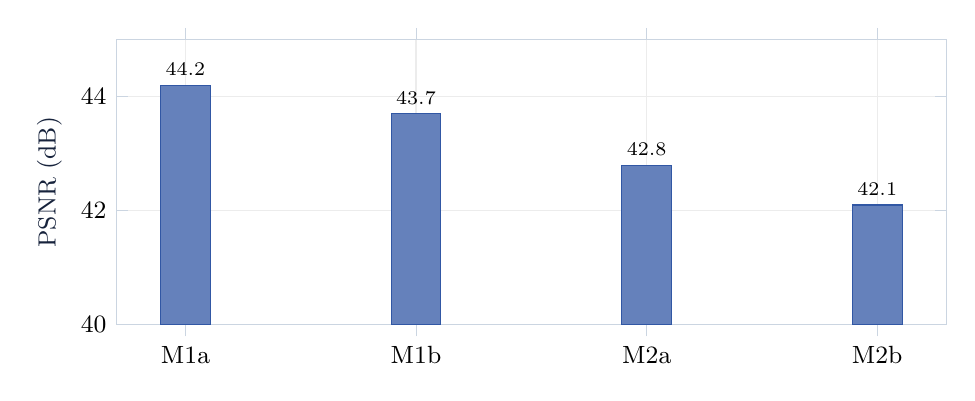
\begin{tikzpicture}
\begin{axis}[width=\columnwidth,height=5.2cm,ybar,bar width=18pt,symbolic x coords={M1a,M1b,M2a,M2b},xtick=data,ylabel={PSNR (dB)},ymin=40,ymax=45,grid=major,grid style={gray!15},nodes near coords,nodes near coords style={font=\scriptsize}]
\addplot[fill=xblue!75,draw=xblue] coordinates {
(M1a,44.2)
(M1b,43.7)
(M2a,42.8)
(M2b,42.1)
};
\end{axis}
\end{tikzpicture}
\caption{Image reference quality (PSNR).}
\end{subfigure}\hfill
\begin{subfigure}{0.49\linewidth}
\centering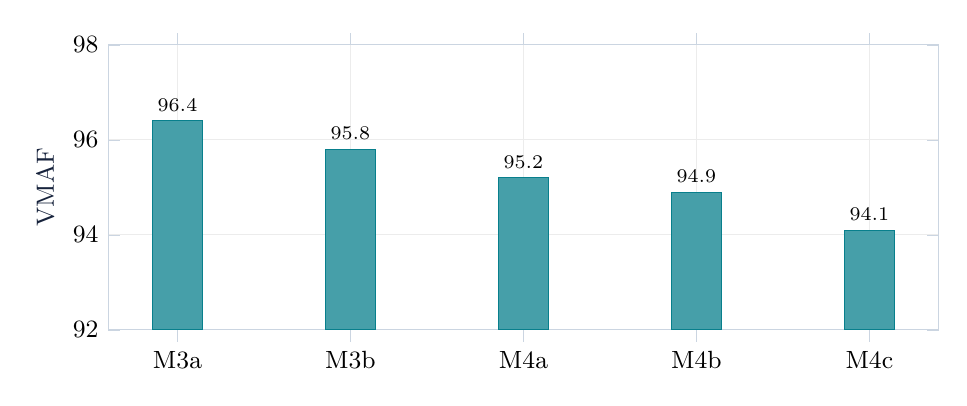
\begin{tikzpicture}
\begin{axis}[width=\columnwidth,height=5.2cm,ybar,bar width=18pt,symbolic x coords={M3a,M3b,M4a,M4b,M4c},xtick=data,ylabel={VMAF},ymin=92,ymax=98,grid=major,grid style={gray!15},nodes near coords,nodes near coords style={font=\scriptsize}]
\addplot[fill=xteal!75,draw=xteal] coordinates {
(M3a,96.4)
(M3b,95.8)
(M4a,95.2)
(M4b,94.9)
(M4c,94.1)
};
\end{axis}
\end{tikzpicture}
\caption{Video reference quality (VMAF).}
\end{subfigure}
\caption{Media-quality measurements beside exact latent equality. PSNR and VMAF use different scales and are plotted separately; neither is a universal perceptual-quality guarantee.}
\label{fig:media-quality}
\end{figure}

The media results cover text-to-image, image-to-image, masked editing, text-to-video, image-to-video, recurrent state, and audio. The MiniMax H3 full run exercised recurrent-state and audio paths. Model licensing remains independent of technical support: some evaluated checkpoints are gated, research-only, or non-commercial.

\subsection{Confidential hardware and relay paths}

Attested L0 ran on four Azure NCC40ads H100 v5 instances in East US 2 with Intel TDX and NVIDIA confidential computing. Attested E4B ran across Google A3 HighGPU TDX and Alibaba gn8v-tee, combining Intel TDX/NVIDIA evidence on Google Cloud and AMD SEV-SNP on Alibaba. Numerical results exactly matched the corresponding commodity Fortress runs. Adversarial tests rejected stale evidence, wrong quotes, second-GPU substitution, and substituted image measurements.

Provider lifecycle tests covered creation, visibility, charge reporting, destruction, and zero remaining instances on all three providers. A complete request also traversed the real Tor network with two relays on hosts separate from the workers; median relay latency was 38 ms above the direct baseline for that measurement.

\subsection{Validation economics and teardown}

The reported total spend was 25,045.91 USD against a 30,000 USD ceiling, leaving 4,954.09 USD unspent. Provider totals were Vast.ai 22,808.62 USD across 179 instances, Azure 353.34 across 9, Google Cloud 521.85 across 7, Alibaba Cloud 243.25 across 5, and RunPod 692.64 across 11+ CPU pods. These are historical charges, not current price quotations.

\begin{figure}[htbp]
\centering
\resizebox{\linewidth}{!}{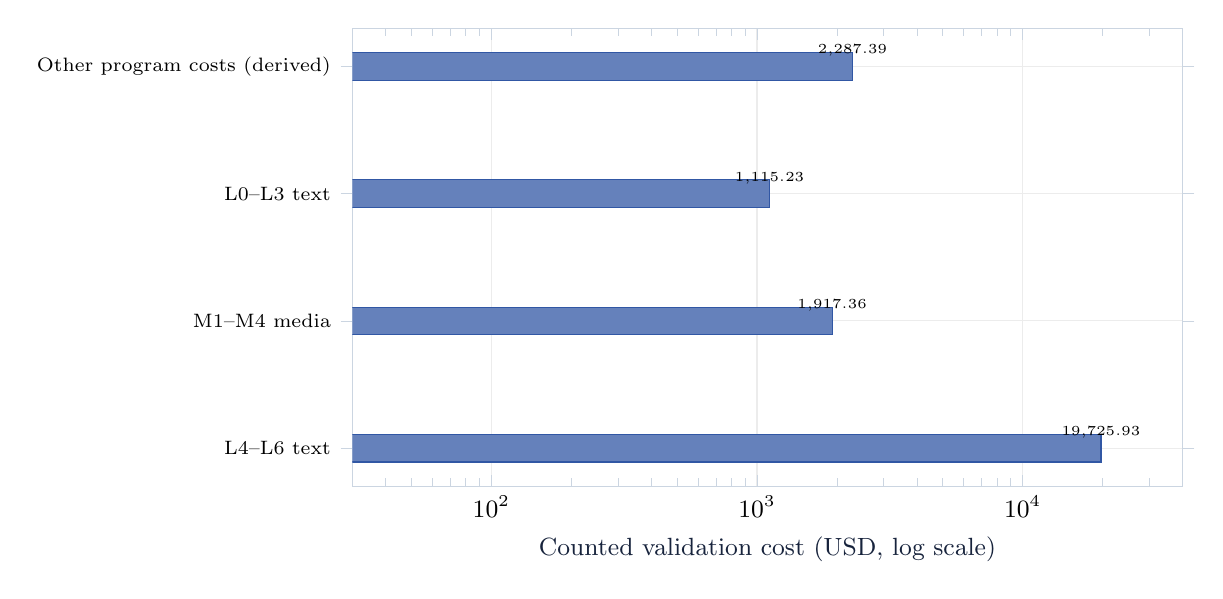
\begin{tikzpicture}
\begin{axis}[width=\columnwidth,height=7.4cm,xbar,xmode=log,log basis x=10,xlabel={Counted validation cost (USD, log scale)},xmin=30,xmax=40000,symbolic y coords={{L4--L6 text},{M1--M4 media},{L0--L3 text},{Other program costs (derived)}},ytick=data,y tick label style={font=\scriptsize},grid=major,grid style={gray!15},nodes near coords,nodes near coords style={font=\tiny,/pgf/number format/fixed},point meta=explicit]
\addplot[fill=xblue!75,draw=xblue] coordinates {
(2287.39,{Other program costs (derived)}) [2287.39]
(1115.23,{L0--L3 text}) [1115.23]
(1917.36,{M1--M4 media}) [1917.36]
(19725.93,{L4--L6 text}) [19725.93]
};
\end{axis}
\end{tikzpicture}}
\caption{Validation cost by broad ladder group. ``Other program costs'' is derived as the published total minus itemized L0--L6 and M1--M4 rung costs, and includes engineering, provider, TEE, teardown, storage, bandwidth, and residual charges.}
\label{fig:costs}
\end{figure}

After execution, workers and relays were stopped, worker exit codes collected, resources destroyed, and provider APIs queried independently. The report records zero remaining instances and volumes at Vast.ai, Azure, Google Cloud, Alibaba Cloud, and RunPod. Final charge reconciliation included storage, bandwidth, and residual costs; a stopped virtual machine was not treated as free or destroyed.

\section{Security evaluation and limitations}\label{sec:security-evaluation}

\subsection{Adversarial validation}

Each hardware rung completed 34 worker-compromise and transport checks. The adversary was granted access to its own worker process, artifacts, and credentials rather than modeled as a blind external observer. Tests covered peer-artifact decryption, boundary-key availability, model and prompt remnants, tampered manifests and shards, stale-epoch mixing, replay, malformed framing, and altered results. Memory and log scans searched for checkpoints, source matrices, embeddings/heads/routers, client bases, VAE material, prompts, and recoverable latents.

Attested executions additionally substituted stale quotes, incorrect evidence, a second GPU, and a changed image measurement. Each was rejected. CUDA forensics on RTX 4090, A100 80 GB, and H100 80 GB exercised scrub-then-probe, zero-on-free/reallocation, and KV/latent/recurrent/transport cleanup; \texttt{compute-sanitizer --tool initcheck} reported clean results for the tested paths.

Zero observed Freivalds failures across accepted rungs means no incorrect result escaped the implemented verification gate in those tests. It does not make the theoretical false-acceptance probability zero. Likewise, passing a fixed attack suite is evidence about those tests and their implementation, not proof that no other attack exists.

\subsection{Formal protocol models}

ProVerif models cover direct and relayed Fortress role sessions over adversary-controlled channels. Queries address request/response secrecy after specified key disclosures and injective agreement on session keys. A relayed model also considers later ratchet-key disclosure. Control runs demonstrate that the models can fail when the corresponding protection is removed.

These are symbolic models, not computational proofs of hybrid ML-KEM/X25519 security. They do not cover every replay window, side channel, TLS implementation, identity compromise, or provider behavior. Known-answer tests use NIST ACVP and Project Wycheproof material for supported post-quantum operations, while round-trip tests cover library-generated randomness.

\subsection{Structural leakage and algebraic obfuscation}

Orthogonal conjugation $W\mapsto UWU^{\top}$ can preserve exact layer behavior, but also preserves norms, inner products, eigenspectra, and other structural quantities. Given public or related models, Procrustes-style alignment and norm analysis can recover information. A basis change therefore supplies computational obfuscation at most; it is not semantically secure encryption, FHE, secret sharing, or a zero-knowledge proof.

Fortress addresses this by making additive sharing the primary confidentiality boundary. The full random variant has an information-theoretic hiding argument under independence and non-collusion. Seed expansion changes the claim to computational hiding. No amount of basis rotation changes that classification.

\subsection{Collusion and placement}

Below-threshold worker collusion was tested and fails to reconstruct protected values. Full-grid collusion remains a residual risk by construction. Placement across countries, CPU vendors, and providers reduces correlated operational control only if the metadata is truthful. Operator-supplied labels are not independently verified proof of legal or organizational independence.

A deployment that places complementary shares on different ports of one host has failed its security objective even if arithmetic remains correct. Similarly, multiple cloud accounts controlled by one operator may not create meaningful independence. Non-collusion is therefore both a protocol assumption and a governance requirement.

\subsection{Traffic and microarchitectural channels}

Fixed frames, cover calls, decoys, padded dispatch, and relays mitigate selected observable signals. They do not establish anonymity against a global passive observer. Entry and exit relays learn endpoint metadata; long-lived constant-rate flows can themselves be recognizable; real requests can exhibit model-dependent operation order. MoE padding equalizes workload size but not necessarily kernel duration, memory addresses, cache/TLB activity, power consumption, or scheduling patterns.

A local leave-one-out nearest-mean timing experiment reported balanced accuracy 0.572 against a 0.5 baseline for one run. This small measurement is not general classifier resistance and should motivate further evaluation rather than a blanket non-leakage claim.

\subsection{TEE and physical limitations}

A TEE adds hardware-enforced isolation and measured identity, but does not remove trust in CPU/GPU vendors, firmware, collateral, or verifier correctness. Probing, fault injection, cold-boot, acoustic/electromagnetic leakage, physical bus attacks, and compromised attestation roots were not tested. NVIDIA and CPU evidence must be bound to the same session and workload to prevent composite substitution.

Even with valid attestation, a measured application can have a vulnerability, and an external verifier service can become unavailable or compromised. TEE mode is an additional barrier whose failure must be explicit, not an unconditional guarantee.

\subsection{Outstanding independent assurance}

The public validation record explicitly leaves the following outside its completed scope:
\begin{itemize}
  \item independent cryptography and systems audit with published findings;
  \item second-party reproducible builds and independently operated public-log witnessing;
  \item a public per-threat comparison with other confidential-computing and MPC systems;
  \item an open red-team or bounty period;
  \item hosted continuous integration on the frozen validated build, which was unavailable because of account billing during validation.
\end{itemize}
These omissions do not invalidate the reported physical tests, but they limit the strength of public assurance. Production acceptance is therefore a scoped engineering decision, not a claim of formal system-wide proof.

\section{Related work}\label{sec:related}

\paragraph{Confidential virtual machines and accelerators.}
AMD SEV-SNP and Intel TDX isolate virtual-machine state from parts of the host stack, while NVIDIA confidential computing extends attestation to supported GPUs~\cite{amd-sev-snp,intel-tdx,nvidia-cc}. These technologies reduce exposure to infrastructure operators but retain vendor, firmware, and verifier trust. Fortress can use them as an additional layer and separately protects operands through sharing on commodity workers.

\paragraph{Secure multiparty computation and homomorphic encryption.}
Secret sharing originates in threshold cryptography~\cite{shamir1979}; modern MPC protocols distribute computation under explicit corruption thresholds. FHE permits computation over encrypted data under cryptographic hardness assumptions~\cite{gentry2009}. Fortress is narrower than general-purpose MPC or FHE: it delegates exact linear maps and leaves nonlinear semantics at the client. This specialization makes GPU implementation practical for the evaluated graphs, but increases client work and requires a non-colluding placement policy.

\paragraph{Verifiable computation.}
Freivalds' randomized matrix-product test is a classical example of efficient algebraic verification~\cite{freivalds1977}. General-purpose succinct arguments can cover broader computations but introduce different setup, proof, and performance costs. Fortress applies the specialized test where its finite-field assumptions hold and does not extrapolate its probability bound to rounded floating-point kernels.

\paragraph{Distributed inference.}
Pipeline and tensor parallelism partition neural-network execution to fit and accelerate large models; GPipe and Megatron-LM are influential examples~\cite{gpipe,megatron}. Serving systems such as vLLM and SGLang optimize scheduling, KV management, and GPU utilization~\cite{vllm,sglang}. These systems ordinarily trust the execution environment with plaintext model state. Fortress uses distributed placement for confidentiality and integrity in addition to capacity, and its protected production engine is distinct from ordinary plaintext serving.

\paragraph{Provider-operated private AI.}
Systems such as Apple Private Cloud Compute emphasize hardware/software transparency and provider-operated attested infrastructure~\cite{apple-pcc}. Fortress instead supports a mixture of independent commodity and confidential workers with client-owned model semantics. A definitive per-threat comparison requires independent analysis; this paper identifies architectural differences without claiming universal superiority.

\paragraph{Private model transformation.}
Basis rotations and related transformations can preserve neural-network behavior while changing representations. Their equivalence equations do not by themselves provide cryptographic confidentiality, particularly when public-weight alignment and invariant attacks are available. Fortress limits these transformations to inner compatibility and compilation mechanisms rather than counting them as its primary security guarantee.

\section{Conclusion}\label{sec:conclusion}

Xurcroh Fortress demonstrates a concrete approach to private distributed inference in which independent GPU workers perform exact quantized linear operations over additive shares, while a trusted client retains the semantic and nonlinear boundaries of the model. Freivalds verification, recipient-isolated artifacts, hybrid post-quantum sessions, fail-closed attestation, memory lifecycle controls, and signed task traces address different parts of the threat model without being conflated into a single unsupported security guarantee.

The reported physical evaluation covers dense, MoE, VLM, image, and video workloads from small RTX 4090 grids to a 120-host H100 fleet, with exact equality to the quantized reference on every published rung. Attested executions across Azure, Google Cloud, and Alibaba Cloud demonstrate that commodity sharing and confidential hardware can be complementary rather than mutually exclusive deployment strategies.

The architecture's costs are equally important. The trusted client performs substantial computation and state management; communication grows with the share grid; large MoE models require large independent fleets; and traffic-analysis, full-collusion, microarchitectural, and physical threats remain. Seed-expanded shares reduce bandwidth but weaken the confidentiality classification from information-theoretic to computational hiding. External audit, second-party reproducibility, independent witnessing, and open adversarial review remain necessary assurance work.

Fortress is therefore best understood as a working, scoped private-inference architecture and an evidence framework: useful not because it claims trust has disappeared, but because it makes precisely visible where trust remains.

\appendix
\section{Mathematical and protocol details}\label{app:math}

\subsection{Exact grid reconstruction}

Expanding \cref{eq:grid} produces all cross terms. Modulo $p$,
\begin{equation}
\sum_{i=1}^{N}\sum_{j=1}^{N}W_iX_j
=\sum_{i=1}^{N}W_i\left(\sum_{j=1}^{N}X_j\right)
=\left(\sum_{i=1}^{N}W_i\right)X=WX.
\end{equation}
No cross term is approximated or discarded. Role order and transport packetization do not affect the exact sum provided field accumulation bounds hold. This proof addresses arithmetic correctness only; confidentiality comes from the distribution and placement of shares, and integrity comes from independent verification.

\subsection{Pseudo-Mersenne reduction}

For a 64-bit product $z$, let $z_0=z\bmod2^{32}$ and $z_1=\lfloor z/2^{32}\rfloor$. Since $2^{32}=p+5$,
\begin{equation}
z=z_0+(p+5)z_1\equiv z_0+5z_1\pmod p.
\end{equation}
The folded value can exceed 32 bits, so the same operation is repeated before final canonical reduction. Any native implementation must account for the wider intermediate produced by $5z_1$; an implementation that merely masks to 32 bits would be incorrect.

\subsection{Challenge composition}

For an incorrect result $C=AB+D$ with $D\neq0$, the verifier computes $Cr-A(Br)=Dr$. If independent random challenges $r_1,\ldots,r_R$ are used, every challenge must land in the zero set of every nonzero row for a false acceptance. Conditional independence gives $\Pr[\mathrm{accept}]\leq p^{-R}$. Reusing a challenge after disclosure or allowing a worker to choose it violates this argument.

\subsection{Client-server work decomposition}

If a layer has $L$ supported linear maps, direct request/response execution incurs on the order of $L$ grid interactions per model invocation, each with $N^2$ roles before batching or parallelism. Let $q_\ell$ denote the elements of activation share $\ell$ and $b$ its encoded byte width. Full activation sharing has total payload proportional to $bN\sum_\ell q_\ell$, while seeded shares replace $N-1$ full payloads with fixed-size seeds and retain one residual payload. The latter reduces bandwidth but changes the security assumption to PRG-based computational hiding.

\subsection{Transform compatibility}

For an orthogonal $Q$, $Q^{-1}=Q^\top$. Conjugating a linear map, $\widehat{W}=Q_{\mathrm{out}}WQ_{\mathrm{in}}^\top$, gives
\begin{equation}
\widehat{W}(Q_{\mathrm{in}}x)=Q_{\mathrm{out}}Wx.
\end{equation}
For attention scores, a shared orthogonal $Q$ preserves $q^\top k=(Qq)^\top(Qk)$ only when no intervening position-dependent operation violates commutation. Rotary positional embeddings impose that adjacent or half-split rotation pairs share the same transform. Grouped-query attention additionally requires consistency within each KV group. These are compatibility conditions for functional equivalence, not evidence of secrecy.

\section{Validated model inventory}\label{app:models}

\Cref{tab:model-inventory} lists the pinned revisions used by the public validation record. Fingerprints and full license notes are available in the repository's model matrix and hardware report.

{\scriptsize
\begin{longtable}{p{0.25\linewidth}p{0.45\linewidth}p{0.09\linewidth}p{0.08\linewidth}}
\caption{Official model checkpoints and immutable revisions used in validation.}\label{tab:model-inventory}\\
\toprule
\textbf{Model} & \textbf{Revision} & \textbf{Encoding} & \textbf{Rung} \\
\midrule
\endfirsthead
\toprule
\textbf{Model} & \textbf{Revision} & \textbf{Encoding} & \textbf{Rung} \\
\midrule
\endhead
\bottomrule
\endfoot
Gemma 4 E2B & \texttt{4adf15748de9e1a0097b6274cee9c15836c41c37} & BF16 & L0/D2 \\
Gemma 4 E4B & \texttt{4ecc2ba63bcac23ba4a767fc87025b1450f84c9c} & BF16 & L1a/D2 \\
Gemma 4 12B & \texttt{43c9d014b231474fa7212dbb48a762566c2b255d} & BF16 & L1b \\
Gemma 4 26B-A4B & \texttt{4d7ae4984b7db7de8f8457170b3f1a419ee76d52} & BF16 & L2 \\
Gemma 4 31B & \texttt{842da3794eaa0b77d5f08bae87a17459d91ff475} & BF16 & L3a \\
Qwen 3.8 27B & \texttt{37561816e66b5b9153b1b64c10968c18c1e6f4a0} & BF16 & L3b \\
Mistral Medium 3.5 128B & \texttt{ff62230e1c990bdf05bbf6efa1c73fefe094ebf4} & FP8 & L4 \\
GLM-5.3-Flash & \texttt{46a050bec13002ad29ee795c16e61cf4fa3c4a9c} & FP8 & L5 \\
Kimi-K2.6 & \texttt{7eb5002f6aadc958aed6a9177b7ed26bb94011bb} & Packed I32 & L6 \\
FLUX.2 klein 4B & \texttt{e7b7dc27f91deacad38e78976d1f2b499d76a294} & BF16 & M1a \\
Z-Image-Turbo & \texttt{f332072aa78be7aecdf3ee76d5c247082da564a6} & BF16 & M1b \\
Qwen-Image 2.1 & \texttt{d26bb61231c349cf6b7896fa83353113880e1ba3} & BF16 & M2a \\
FLUX.2-dev & \texttt{e8af80c9dd820ab07ee4171d024f03e5c4b3024b} & BF16 & M2b \\
Wan 2.2 TI2V 5B & \texttt{b8fff7315c768468a5333511427288870b2e9635} & BF16 & M3a \\
LTX-2.5 & \texttt{4791a1100e0cf97f7ed5c55c12dd71dce13f9dd3} & BF16 & M3b \\
Wan 2.2 T2V-A14B & \texttt{5be7df9619b54f4e2667b2755bc6a756675b5cd7} & BF16 & M4a \\
Wan 2.2 I2V-A14B & \texttt{596658fd9ca6b7b71d5057529bbf319ecbc61d74} & BF16 & M4b \\
MiniMax H3 & \texttt{12253298adb81e36757eabebb81d2ba1c0cc70cc} & BF16 & M4c \\
\end{longtable}}

\section{Evidence and acceptance matrix}\label{app:evidence}

\begin{table}[htbp]
\centering\small
\caption{Evidence classes used in this paper.}
\begin{tabularx}{\linewidth}{p{0.22\linewidth}XX}
\toprule
\textbf{Class} & \textbf{Meaning} & \textbf{Examples} \\
\midrule
Formally derived & Follows from explicit algebra and assumptions & Grid reconstruction; single-share hiding; finite-field Freivalds bound \\
Locally validated & Executed in CPU/local test or symbolic analysis & Decoder differentials; protocol parsing; ProVerif queries; arithmetic experiment \\
Hardware validated & Observed on the stated physical frozen build & L0--L6, M1--M4; three-provider attestation; memory forensics \\
Governance decision & Acceptance by the responsible project owner & Production acceptance under report conditions \\
External pending & Requires another party or public process & Audit; second-party builds; independent witness; bounty/red team \\
\bottomrule
\end{tabularx}
\end{table}

The signed validation chain orders F0, M0, G2, G3, G4, G5, G6, M1, M2, M3, M4, G11, G12, G13, D2-a, and D2-b. Each record identifies its predecessor and source revision. Public report examples include F0 SHA-256 \path{b42f0a9c31d5e8774a6c0091b2e358f41e0d7c3992ab6451c45e0a2b8d91f302} and L6 SHA-256 \path{e9031d1cc44a0f2b775e6b8f0a2d913e5c7044ab1d22ef6689c0d1e3f445a6b7}.

\section{Artifact guide}\label{app:artifact}

The repository contains the public SDK under \path{python/Xurcroh}, the internal Python runtime under \path{python/xurcroh}, Rust protocol/crypto/transport crates under \path{crates}, native CUDA code under \path{native/cuda}, executable tests under \path{tests}, and the independent interactive manual under \path{apps/web-manual}. Deployment guides cover Vast.ai, RunPod, Azure confidential GPUs, and Google Cloud confidential GPUs.

Build this manuscript from the repository root:
\begin{lstlisting}[language=bash]
./scripts/build-paper.sh
\end{lstlisting}
Regenerate local arithmetic evidence and run its tests:
\begin{lstlisting}[language=bash]
.venv/bin/python experiments/fortress_arithmetic.py --iterations 5
.venv/bin/pytest tests/fortress tests/experiments/test_fortress_arithmetic.py -q
\end{lstlisting}

No model checkpoint, private key, raw prompt, source media, generated output, or provider credential is needed to rebuild the paper. Hardware-run reproduction requires separately authorized infrastructure and compliance with each model's license.

\printbibliography
\end{document}
